\documentclass[leqno]{book}
\usepackage[dvipsnames,svgnames]{xcolor}
\usepackage{colortbl}
\usepackage{graphicx}
\graphicspath{{./figure/}}
\usepackage{geometry}
\geometry{b5paper,left=1in,right=1in,top=0.75in,bottom=0.75in}%标准的Microsoft Word 文档页面
\usepackage{multicol}
\usepackage{array}
\usepackage{indentfirst}
%\setlength{\parindent}{2em}%设置段首缩进
\linespread{1.5}%行距

%公式
\usepackage{amsmath}
\usepackage{amsfonts}
\usepackage{amssymb}
\usepackage{physics}
\usepackage{tikz-cd}
\usepackage{mathrsfs}

%表格
\usepackage{booktabs}
\usepackage{diagbox}
\usepackage{multirow}
\usepackage{makecell}
\usepackage{longtable}
\usepackage{tabularx}

%谱序列
\usepackage{spectralsequences}

%索引和参考文献
\usepackage[xindy,splitindex]{imakeidx}
%\makeindex[
%	columns=2,
%	program=truexindy,
%	intoc=true,
%	options=-M texindy -I xelatex -C utf8,
%	title={}]
%\addbibresource{}

%实现超链接添加
\usepackage[colorlinks,linkcolor=blue,citecolor=blue]{hyperref}

% 设置 PDF 文件信息
\hypersetup{
	pdfauthor = {},
	pdftitle = {K-Theory},
	pdfkeywords = {},
	CJKbookmarks = true}

%页眉页脚
\usepackage{fancyhdr}
\fancypagestyle{plain}{
	\pagestyle{fancy}
}
\pagestyle{fancy}
\renewcommand{\headrulewidth}{0pt}
%分别填入左中右页眉和左中右页脚,页脚默认为页码/总页数
\lhead{}
\chead{}
\rhead{}
\lfoot{}
\cfoot{}
\rfoot{\thepage} % Counts the pages.

%自定义公式编号
\usepackage{amsthm}
\numberwithin{equation}{section}
\renewcommand{\theequation}{\thesection .\arabic{equation}}

\newtheorem{theorem}{Theorem}[section]%使用\begin{thm}开始新命题,按节编号
\newtheorem{proposition}[theorem]{Proposition}
\newtheorem{corollary}[theorem]{Corollary}
\newtheorem{lemma}[theorem]{Lemma}
\theoremstyle{definition}
\newtheorem{example}[theorem]{Example}
\newtheorem{definition}[theorem]{Definition}
\newtheorem*{solu}{Solution}
\newtheorem*{note}{Note}
\newtheorem*{remark}{Remark}
\newenvironment*{solution}{\begin{solu}}{\hfill\qedsymbol\end{solu}}

%改变强调方式
\renewcommand{\emph}{\textbf}

%多样化目录
%\usepackage{titletoc}
\setcounter{secnumdepth}{3}
\setcounter{tocdepth}{3}


\title{K-Theory}
\author{M. F. Atiyah}

\begin{document}
    \begin{titlepage}
      \vspace*{1cm}
      {\huge\raggedright $K$-Theory\par}
      \noindent\hrulefill\par
      {\LARGE\raggedleft M. F. Atiyah\par}
      \vfill
      {\Large\raggedleft \LaTeX version typed by \href{redenduster@163.com}{Christopher Chou}.\par}
    \end{titlepage}
    \tableofcontents
    \setcounter{chapter}{1}
    \chapter{K-Theory}
        \section{Definitions}
            If $X$ is any space, the set $\operatorname{Vect}(X)$ has the structure of an abelian semigroup, where the additive structure is defined by direct sum. If $A$ is any abelian semigroup, we can associate to $A$ an abelian group $K(A)$ with the following property: there is a semigroup homomorphism $\alpha:A\to K(A)$ such that if $G$ is any group, $\gamma:A\to G$ any semigroup homomorphism, there is a unique homomorphism $\kappa:K(A)\to G$ such that $\gamma=\kappa \alpha$. If such a $K(A)$ exists, it must be unique.

            The group $K(A)$ is defined in the usual fashion. Let $F(A)$ be the free abelian group generated by the elements of $A$, let $E(A)$ be the subgroup of $F(A)$ generated by those elements of the form $a+a'-(a \oplus a')$, where $\oplus $ is the addition in $A$, $a,a'\in A$. Then $K(A)=F(A)/E(A)$ has the universal property described above, with $\alpha:A\to K(A)$ being the obvious map.

            A slightly different construction of $K(A)$ which is sometimes convenient is the following. Let $\Delta:A\to A\times A$ be the diagonal homomorphism of semi-groups, and let $K(A)$ denote the set of cosets of $\Delta(A)$ in $A\times A$. It is a quotient semi-group, but the interchange of factors in $A\times A$ induces an inverse in $K(A)$ so that $K(A)$ is a group. We then define $\alpha _{A}:A\to K(A)$ to be the composition of $a\to (a,0)$ with the natural projection $A\times A\to K(A)$ (we assume $A$ has a zero for simplicity). The pair $(K(A),\alpha _{A})$ is a functor of $A$ so that if $\gamma:A\to B$ is a semi-group homomorphism we have a commutative diagram
            \begin{equation*}
                \begin{tikzcd}
                    A \arrow[d, "\gamma"'] \arrow[r, "\alpha_A"] & K(A) \arrow[d, "K(\gamma)"] \\
                    B \arrow[r, "\alpha_B"]                      & K(B)                       
                \end{tikzcd}
            \end{equation*}
            If $B$ is a group $\alpha _{B}$ is an isomorphism. That shows $K(A)$ has the required universal property.

            If $A$ is also a semi-ring (that is, $A$ possesses a multiplication which is distributive over the addition of $A$) then $K(A)$ is clearly a ring.

            If $X$ is a space, we write $K(X)$ for the ring $K(\operatorname{Vect}(X))$. No confusion should result from this notation. If $E\in \operatorname{Vect}(X)$, we shall write $[E]$ for the image of $E$ in $K(X)$. Eventually, to avoid excessive notation, we may simply write $E$ instead of $[E]$ when there is no danger of confusion.

            Using our second construction of $K$ it follows that, if $X$ is a space, every element of $K(X)$ is of the form $[E]-[F]$, where $E,F$ are bundles over $X$. Let $G$ be a bundle such that $F \oplus G$ is trivial. We write $\underline{n}$ for the trivial bundle of dimension $n$. Let $F \oplus G = \underline{n}$. Then $[E]-[F]=[E]+[G]-([F]+[G])=[E\oplus G]-[\underline{n}]$. Thus, every element of $K(X)$ is of the form $[H]-[\underline{n}]$.

            Suppose the $E,F$ are such that $[E]=[F]$, then again from our second construction of $K$ it follows that there is a bundle $G$ such that $E\oplus G\simeq F\oplus G$. Let $G'$ be a bundle such that $G\oplus G'=\underline{n}$. Then $E\oplus G\oplus G'\simeq F\oplus G\oplus G'$, so $E\oplus \underline{n}\simeq F\oplus \underline{n}$. If two bundles become equivalent when a suitable trivial bundle is added to each of them, the bundles are said to be \emph{stably equivalent}. Thus, $[E]=[F]$ if and only if $E$ and $F$ are stably equivalent.

            If we define $\operatorname{Vect}_{n}(X)\to \operatorname{Vect}_{n+1}(X)$ by the addition of a trivial line-bundle it follows that we have
            \begin{lemma}
                For a compact connected space $X$,
                \begin{equation*}
                  K(X)\simeq \mathbb{Z}\times \varinjlim_{n} \operatorname{Vect}_{n}(X)
                \end{equation*}
            \end{lemma}

            Suppose $f:X\to Y$ is a continuous map. Then $f^{*}:\operatorname{Vect}(Y)\to \operatorname{Vect}(X)$ induces a ring homomorphism $f^{*}:K(Y)\to K(X)$. By $(1.4.3)$ this homomorphism depends only on the homotopy class of $f$.

            We conclude this section by giving the homotopy-theoretic definition of $K(X)$. This is essentially a re-interpretation of the results on $\operatorname{Vect}_{n}(X)$ in Chapter \uppercase\expandafter{\romannumeral 1}. We introduce the "infinite" unitary group $U$ defined as
            \begin{equation*}
              U=\varinjlim_{n}U(n)
            \end{equation*}
            under the standard inclusions. Correspondingly for the classifying spaces we have
            \begin{equation*}
              BU=\varinjlim_{n}BU(n).
            \end{equation*}
            Recall also that the classifying space $BU(n)$ can be taken to be the limit Grassmannian:
            \begin{equation*}
              BU(n)=\varinjlim_{m}G_{n}(C^{m}).
            \end{equation*}
            Hence from Theorem 1.4.15, for any compact connected $X$, we have
            \begin{equation*}
                \begin{aligned}
                    [X,BU]&=\varinjlim_{n}[X,BU(n)] \\
                    &= \varinjlim_{n}\varinjlim_{m}[X,G_{n}(C^{m})] \\
                    &= \varinjlim_{n} \operatorname{Vect}_{n}(X) \\
                    &= \tilde{K}(X) \qquad \text{by (2.1.1)}
                \end{aligned}
            \end{equation*}
            Equivalently, for all compact $X$, we have
            \setcounter{theorem}{9}
            \begin{proposition}
              $K(X)\simeq [X,\mathbb{Z}\times BU]$.
            \end{proposition}

            Similarly, (2.17) can be written as
            \begin{proposition}
              $\tilde{K}(SX)\simeq [X,U]$.
            \end{proposition}

            In fact 2.1.11 is a consequence of 2.1.10 and the homotopy equivalence
            \begin{equation*}
              U\sim \Omega BU.
            \end{equation*}
            More generally we have for all $n\geq 1$
            \begin{proposition}
              $K^{-n}(X)\simeq [X,\Omega^{n}BU]\simeq [X,\Omega^{n-1}U]$.
            \end{proposition}

        \section{Elementary Properties}
        
            We next define relative groups $K(X,Y)$ for a compact pair $(X,Y)$, with $Y \subset X$.

            Let $\mathcal{C}$ denote the category of compact spaces, $\mathcal{C}^{+}$ the category of compact spaces with distinguished basepoint, and $\mathcal{C}^{2}$ the category of compact pairs. We define functors:
            \begin{equation*}
              \begin{aligned}
              \mathcal{C}^{2}\to \mathcal{C}^{+} \\
              \mathcal{C}\to \mathcal{C}^{2}
              \end{aligned}
            \end{equation*}
            by sending a pair $(X,Y)$ to $X/Y$ with basepoint $Y/Y$ (if $Y=\varnothing$, the empty set, $X/Y$ is understood to be the disjoint union of $X$ with a point.) We send a space $X$ to the pair $(X,\varnothing)$. The composite $\mathcal{C}\to \mathcal{C}^{+}$ is given by $X\to X^{+}$, where $X^{+}$ denotes $X/\varnothing$.

            If $X$ is in $\mathcal{C}^{+}$, we define $\tilde{K}(X)$ to be the kernel of the map $i^{*}: K(X)\to K(x_{0})$ where $i:x_{0}\to X$ is the inclusion of the basepoint. If $c:X\to x_{0}$ is the collapsing map then $c^{*}$ induces a splitting $K(X)\simeq \tilde{K}(X)\oplus K(x_0)$. This splitting is clearly natural for maps in $\mathcal{C}^{+}$. Thus $\tilde{K}$ is a functor on $\mathcal{C}^{+}$. Also, it is clear that $K(X)\simeq \tilde{K}(X^{+})$. We define $K(X,Y)$ by $K(X,Y)=\tilde{K}(X/Y)$. In particular $K(X,\varnothing)\simeq K(X)$. Since $\tilde K$ is a functor on $\mathcal{C}^{+}$ it follows that $K(X,Y)$ is a contravariant functor of (X,Y) in $\mathcal{C}^{2}$.

            We now introduce the "smash product" operation in $\mathcal{C}^{+}$. If $X,Y\in \mathcal{C}^{+}$ we put 
            \begin{equation*}
              X\wedge Y=X\times Y/X\vee Y
            \end{equation*}
            where $X\vee Y=X\times y_0\cap x_{0}\times Y$, $x_0,y_0$ being the base-points of $X,Y$ respectively. For any three spaces $X,Y,Z \in \mathcal{C}^{+}$ we have a natural homeomorphism
            \begin{equation*}
              X\wedge (Y\wedge Z)\approx (X\wedge Y)\wedge Z
            \end{equation*}
            and we shall identify these spaces by the homeomorphism.

            Let $I$ denote the unit interval $[0,1]$ and let $\partial I=\{0\}\cup \{1\}$ be its boundary. We take $I/\partial I\in \mathcal{C}^{+}$ as our standard model of the circle $S^{1}$. Similarly if $I^{n}$ denotes the unit cube in $\mathbb{R}^{n}$ we take $I^{n}/\partial I^{n}$ as our model of the $n$-sphere $S^{n}$. Then we have a natural homeomorphism
            \begin{equation*}
              S^{n}\simeq S^{1}\wedge S^{1}\wedge \cdots \wedge S^{1} \qquad \text{(n factors)}.
            \end{equation*}
            For $X \in \mathcal{C}^{+}$ the space $S^{1}\wedge X \in \mathcal{C}^{+}$ is called the \emph{reduced suspension} of $X$, and often written as $SX$. The $n$-th iterated suspension $SS\cdots SX$ ($n$ times) is naturally homeomorphic to $S^{n}\wedge X$ and is written briefly as $S^{n}X$.

            \setcounter{theorem}{1}
            \begin{definition}
              For $n \geq 0$
              \begin{equation*}
                \begin{aligned}
                  &\tilde{K}^{-n}(X) &= \tilde{K}(S^{n}X) & &\text{for }X \in \mathcal{C}^{+} \\
                  &K^{-n}(X,Y) &= \tilde{K}^{-n}(X/Y) &= \tilde{K}(S^{n}(X/Y)) &\text{for }(X,Y)\in \mathcal{C}^{2} \\
                  &K^{-n}(X) &= K^{-n}(X,\varnothing) &= \tilde{K}(S^{n}(X^{+})) &\text{for } X \in \mathcal{C}.
                \end{aligned}
              \end{equation*}
            \end{definition}

            It is clear that all these are contravariant functors on the appropriate categories.

            Before proceeding further we define the \emph{cone on} $X$ by
            \begin{equation*}
              CX = I\times X/\{0\}\times X.
            \end{equation*}
            Thus $C$ is a functor $C:\mathcal{C}\to \mathcal{C}^{+}$. We identify $X$ with the subspace $\{1\}\times X$ of $CX$. The space $CX/X=I\times X / \partial I\times X$ is called the \emph{unreduced suspension} of $X$. Note that this is a functor $\mathcal{C}\to \mathcal{C}^{+}$ whereas the reduced suspension $S$ is a functor $\mathcal{C}^{+}\to \mathcal{C}^{+}$. If $X \in \mathcal{C}^{+}$ with base-point $x_{0}$ then we have a natural inclusion map
            \begin{equation*}
              I \approx Cx_0/x_0 \to CX/X 
            \end{equation*}
            and the quotient space obtained by collapsing $I$ in $CX / X$ is just $SX$. Thus by (1.4.8) $p:CX /X \to SX$ induces an isomorphism $K(SX)\simeq K(CX / X)$ and hence also an isomorphism $\tilde{K}(SX)\simeq K(CX,X)$. Thus the use of $SX$ for both the reduced and unreduced suspensions leads to no problems.

            If $(X,Y) \in C^{2}$ we define $X\cup CY$ to be the space obtained from $X$ and $CY$ identifying the subspaces $Y \subset X$ and $\{1\}\times Y \subset CY$. Taking the base-point of $CY$ as base-point of $X\cup CY$ we have
            \begin{equation*}
              X\cup CY \in \mathcal{C}^{+}.
            \end{equation*}

            We note that $X$ is a subspace of $X\cup CY$ and that there is a natural homeomorphism
            \begin{equation*}
              (X \cup CY)/X \approx CY /Y.
            \end{equation*}
            Thus, if $Y\in \mathcal{C}^{+}$,
            \begin{equation*}
              \begin{aligned}
              K(X\cup CY,X) &\simeq K(CY,Y) \\
              &\simeq \tilde{K}(SY) \\
              &= \tilde{K}^{-1}(Y).
              \end{aligned}
            \end{equation*}

            Now we begin with a simple lemma
            \begin{lemma}
              For $(X,Y)\in \mathcal{C}^{2}$ we have an exact sequence
              \begin{equation*}
                K(X,Y)\stackrel{j^{*}}{\rightarrow}K(X)\stackrel{i^{*}}{\rightarrow}{K(Y)}
              \end{equation*}
              where $i:Y\to X$ and $j:(X,\varnothing)\to (X,Y)$ are the inclusions.
            \end{lemma}

            \begin{proof}
              The composition $i^{*}j^{*}$ is induced by the composition $ji:(Y,\varnothing)\to (X,Y)$, and so factors through the zero group $K(Y,Y)$. Thus $i^{*}j^{*}=0$. Suppose now that $\xi \in \operatorname{Ker} i^{*}$. We may represent $\xi$ in the form $[E]-[n]$ where $E$ is a vector bundle over $X$. Since $i^{*}\xi=0$ it follows that $[E|_{Y}]=[n]$ in $K(Y)$. This implies that for some integer $m$ we have
              \begin{equation*}
                (E\oplus m)|_{Y}=n\oplus m
              \end{equation*}
              i.e., we have a trivialization $\alpha$ of $(E\oplus m)|_{Y}$. This defines a bundle $E\oplus m/\alpha$ on $X/Y$ and so an element
              \begin{equation*}
                \eta=[E\oplus m/\alpha]-[n\oplus m] \in \tilde{K}(X/Y)=K(X,Y).
              \end{equation*}
              Then
              \begin{equation*}
                \begin{aligned}
                  j^{*}(\eta)&=[E\oplus m]-[n\oplus m] \\
                  &=[E]-[n]=\xi.
                \end{aligned}
              \end{equation*}
              Thus $\operatorname{Ker} i^{*}=\operatorname{Im} j^{*}$ and the exactness is established.
            \end{proof}

            \begin{corollary}
              If $(X,Y)\in \mathcal{C}^{2}$ and $Y \in \mathcal{C}^{+}$ (so that, taking the same base-point of $X$, we have $X \in \mathcal{C}^{+}$ also), then the sequence
              \begin{equation*}
                K(X,Y)\to \tilde{K}(X)\to \tilde{K}(Y)
              \end{equation*}
              is exact.
            \end{corollary}

            \begin{proof}
              This is immediate from (2.2.3) and the natural isomorphisms
              \begin{equation*}
                \begin{aligned}
                K(X) \simeq \tilde{K}(X)\oplus K(y_0) \\
                K(Y)\simeq \tilde{K}(Y)\oplus K(y_0).
                \end{aligned}
              \end{equation*}
            \end{proof}
            
            We are now ready for our main proposition:
            \begin{proposition}
              For $(X,Y)\in \mathcal{C}^{+}$ there is a natural exact sequence (infinite to the left)
              \begin{equation*}
                \begin{tikzcd}
                  \cdots K^{-2}(Y) \arrow[r, "\delta"] & K^{-1}(X,Y) \arrow [r, "j^{*}"] & K^{-1}(X) \arrow[r, "i^{*}"] & K^{-1}(Y) \arrow [r, "\delta"]  & K^{0}(X,Y)\\
                  \quad \arrow[r, "j^{*}"] & K^{0}(X) \arrow[r, "i^{*}"] & K^{0}(Y).
                \end{tikzcd}
              \end{equation*}
            \end{proposition}

            \begin{proof}
              First we observe that it is sufficient to show that, for $(X,Y)\in \mathcal{C}^{2}$ and $Y \in \mathcal{C}^{+}$, we have an exact sequence of five terms
                \begin{equation}              
                  \tag{*}
                  \begin{tikzcd}
                   \tilde{K}^{-1}(X) \arrow[r, "i^{}"] & \tilde{K}^{-1}(Y) \arrow[r, "\delta"] & \tilde{K}^{0}(X,Y) \arrow[r, "j^{}"] & \tilde{K}^{0}(X)\arrow [r, "i^{*}"] & \tilde{K}^{0}(Y). 
                  \end{tikzcd}
                \end{equation}
              In fact, if this has been established then, replacing $(X,Y)$ by $(S^{n}X,S^{n}Y)$ for $n=1,2, \ldots $ we obtain an infinite sequence continuing ($*$). Then replacing $(X,Y)$ by $(X^{+},Y^{+})$ where $(X,Y)$ is any pair in $\mathcal{C}^{2}$ we get the infinite sequence of the enunciation. Now (2.2.4) gives the exactness of the last three terms of ($*$). To get exactness at the remaining places we shall apply (2.2.4) in turn to the pairs $(X\cap CY,X)$ and $((X\cup CY)\cup CX,X\cup CY)$. First, taking the pair $(X\cup CY,X)$ we get an exact sequence (where $k,m$ are the natural inclusions)
              \begin{equation*}
                \begin{tikzcd}
                  K(X\cup CY,X)\arrow[r, "m^{*}"] & \tilde{K}(X\cup CY)\arrow[r, "k^{*}"] & \tilde{K}(X).
                \end{tikzcd}
              \end{equation*}
              Since $CY$ is contractible, (1.4.8) implies that
              \begin{equation*}
                p^{*}:\tilde{K}(X/Y)\to \tilde{K}(X\cup CY)
              \end{equation*}
              is an isomorphism where
              \begin{equation*}
                p:X\cup CY\to X\cup CY/CY=X/Y
              \end{equation*}
              is the collapsing map. Also the composition $k^{*}p^{*}$ coincides with $j^{*}$. Let
              \begin{equation*}
                \theta:K(X\cup CY,X)\to K^{-1}(Y)
              \end{equation*}
              be the isomorphism introduced earlier. Then defining
              \begin{equation*}
                \delta:K^{-1}(Y)\to K(X,Y)
              \end{equation*}
              by $\delta=m^{*}\theta^{-1}$ we obtain the exact sequence
              \begin{equation*}
                \begin{tikzcd}
                  \tilde{K}^{-1}(Y)\arrow[r, "\delta"] & K(X,Y)\arrow[r, "j^{*}"] & \tilde{K}(X)
                \end{tikzcd}
              \end{equation*}
              which is the middle part of ($*$).

              Finally, we apply (2.2.4) to the pair
              \begin{equation*}
                (X\cup C_1 Y\cup C_2 X,X\cup C_1 Y)
              \end{equation*}
              where we have labelled the cones $C_1$ and $C_2$ in order to distinguish between them. (see figure).

              \tikzset{every picture/.style={line width=0.75pt}} %set default line width to 0.75pt        

              \begin{figure}[htbp]
                \centering
                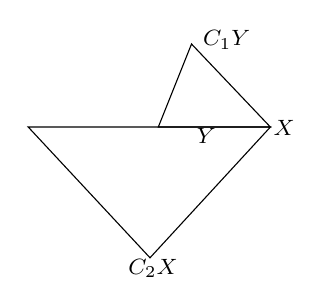
\begin{tikzpicture}[x=0.75pt,y=0.75pt,yscale=-1,xscale=1]
                  %uncomment if require: \path (0,300); %set diagram left start at 0, and has height of 300

                  %Shape: Triangle [id:dp16644158236843398] 
                  \draw   (306.67,186) -- (364.67,123) -- (248,123) -- cycle ;
                  %Shape: Triangle [id:dp40211013265265283] 
                  \draw   (326.67,83) -- (364.67,123) -- (310.67,123) -- cycle ;

                  % Text Node
                  \draw (331,75.4) node [anchor=north west][inner sep=0.75pt]  [font=\footnotesize]  {$C_{1} Y$};
                  % Text Node
                  \draw (328,122.4) node [anchor=north west][inner sep=0.75pt]  [font=\footnotesize]  {$Y$};
                  % Text Node
                  \draw (365,118.4) node [anchor=north west][inner sep=0.75pt]  [font=\footnotesize]  {$X$};
                  % Text Node
                  \draw (295,185.4) node [anchor=north west][inner sep=0.75pt]  [font=\footnotesize]  {$C_{2} X$};
                \end{tikzpicture}
              \end{figure}
              Thus we obtain an exact sequence
              \begin{equation*}
                \begin{tikzcd}
                  K(X\cup C_1 Y\cup C_2 X, X\cup C_1 Y)\arrow[r] & \tilde{K}(X\cup C_1 Y\cup C_2 X)\arrow[r] & \tilde{K}(X\cup C_1 Y).
                \end{tikzcd}
              \end{equation*}
              It will be sufficient to show that this sequence is isomorphic to the sequence obtained from the first three terms of ($*$). In view of the definition of $\delta$ it will be sufficient to show that the diagram
              \begin{equation*}
                \tag{D}
                \begin{tikzcd}
                  {K(X\cup C_1 Y\cup C_2 X, X\cup C_1 Y)} \arrow[rr] \arrow[d, equal] &  & \tilde{K}(X\cup C_1 Y \cup C_2 X) \arrow[d, equal] \\
                  \tilde{K}(C_2 X/X) \arrow[d, equal]                                 &  & \tilde{K}(C_1 Y/Y) \arrow[d, equal]                \\
                  K^{-1}(X) \arrow[rr, "i^{*}"]                                                     &  & K^{-1}(Y)                                                       
                \end{tikzcd}
              \end{equation*}
              commutes up to sign. The difficulty lies, of course, in the fact that $i^{*}$ is induced by the inclusion
              \begin{equation*}
                C_2 Y\to C_2 X
              \end{equation*}
              and that in the above diagram we have $C_1 Y$ and not $C_2 Y$. To deal with this situation we introduce the double cone on $Y$ namely $C_1 Y \cap C_2 Y$. This fits into the commutative diagram of maps
              \begin{equation*}
                \tag{E}
                \begin{tikzcd}
                  X\cup C_1 Y\cup C_2 X \arrow[dd] \arrow[rr, Rightarrow] &                                                                                                  & C_1 Y/Y \arrow[r, Rightarrow]            & SY \\
                                                                          & C_1 Y \cup C_2 Y \arrow[ld] \arrow[lu, Rightarrow] \arrow[rd, Rightarrow] \arrow[ru, Rightarrow] &                                          &    \\
                  C_2 X/X                                                 &                                                                                                  & C_2 Y/Y \arrow[ll] \arrow[r, Rightarrow] & SY
                \end{tikzcd}
              \end{equation*}
              where all double arrows $\Rightarrow$ induce isomorphism in $K$. Using this diagram we see that diagram (D) will commute up to sign provided that the diagram induced by (E)
              \begin{equation*}
                \begin{tikzcd}
                  & K(C_1 Y/Y) \arrow[ld] & \tilde{K}(SY) \arrow[dd, equal] \arrow[l] \\
                  K(C_1 Y \cup C_2 Y) &                       &                                                         \\
                  & K(C_2 Y/Y) \arrow[lu] & \tilde{K}(SY) \arrow[l]                                
                \end{tikzcd}
              \end{equation*}
              commutes up to sign. This will follow at once from the following lemma which is in any case of independent interest and will be needed later.
            \end{proof}

            \begin{lemma}
              Let $T:S^1\to S^1$ be defined by $T(t)=1-t , t\in I$ (we recall that $S^{1}=I/\partial I$) and let $T\wedge I:SY\to SY$ be the map induced by $T$ on $S^1$ and the identity on $Y$ (for $Y\in \mathcal{C}^{+}$). Then $(T\wedge 1)^{*}y=-y$ for $y \in \tilde{K}(SY)$.
            \end{lemma}

            This lemma in turn is an easy corollary of the following:
            \begin{lemma}
              For any map $f:Y\to \operatorname{GL}(n,\mathbb{C})$ let $E_{f}$ denote the corresponding vector bundle over $SY$. Then $f\to [E_{f}]-[n]$ induces a group isomorphism
              \begin{equation*}
                \lim_{n \to \infty}[Y,\operatorname{GL}(n,\mathbb{C})]\simeq \tilde{K}(SY)
              \end{equation*}
              where the group structure on the left is induced from that of $\operatorname{GL}(n,\mathbb{C})$.
            \end{lemma}

            In fact, the operation $(T\wedge 1)^{*}$ on $\tilde{K}(SY)$ corresponds by the isomorphism of (2.2.7) to the operation of replacing the map $y\to f(y)$ by $y\to f(y)^{-1}$, i.e., it corresponds to the inverse in the group. Thus (2.2.7) implies (2.2.6) and hence (2.2.5). It remains therefore to establish (2.2.7). Now (1.4.9) implies that $f\to [E_{f}]-[n]$ induces a bijection of sets
            \begin{equation*}
              \lim [Y,\operatorname{GL}(n,\mathbb{C})]\to \tilde{K}(SY).
            \end{equation*}
            The fact that this is in fact a group homomorphism follows from the homotopy connecting the two maps $\operatorname{GL}(n)\times \operatorname{GL}(n)\to \operatorname{GL}(2n)$ given by
            \begin{equation*}
              A\times B\to \left( \begin{matrix}
                A&		0\\
                0&		B\\
              \end{matrix} \right) 
            \end{equation*}
            and
            \begin{equation*}
              A\times B\to 
              \left( \begin{matrix}
                AB&		0\\
                0&		1\\
              \end{matrix} \right) .
            \end{equation*}
            This homotopy is given explicitly by
            \begin{equation*}
              \rho_{t}(A\times B)=
              \left( \begin{matrix}
                A&		0\\
                0&		1\\
              \end{matrix} \right) \left( \begin{matrix}
                \cos t&		\sin t\\
                -\sin t&		\cos t\\
              \end{matrix} \right) \left( \begin{matrix}
                1&		0\\
                0&		B\\
              \end{matrix} \right) \left( \begin{matrix}
                \cos t&		\sin t\\
                \sin t&		\cos t\\
              \end{matrix} \right) 
            \end{equation*}
            where $0\le t\le \pi/2$.

            From (2.2.5) we deduce at once:

            \begin{corollary}
              If $Y$ is a retract of $X$, then for all $n\ge 0$, the sequence $K^{-n}(X,Y)\to K^{-n}(X)\to K^{-n}(Y)$ is a split short exact sequence, and
              \begin{equation*}
                K^{-n}(X)\simeq K^{-n}(X,Y)\oplus K^{-n}(Y).
              \end{equation*}
            \end{corollary}

            \begin{corollary}
              If $X,Y$ are two spaces with basepoints, the projection maps $\pi_{X}:X\times Y\to X$, $\pi_{Y}:X\times Y\to Y$ induce an isomorphism for all $n\ge 0$
              \begin{equation*}
                \tilde{K}^{-n}(X\times Y)\simeq \tilde{K}^{-n}(X\wedge Y)\oplus \tilde{K}^{-n}(X)\oplus \tilde{K}^{-n}(Y).
              \end{equation*}
            \end{corollary}
            \begin{proof}
              X is a retract of $X\times Y$, and $Y$ is a retract of $(X\times Y)/X$. The result follows by two applications of (2.2.8).
            \end{proof}

            Since $\tilde{K}^{0}(X\wedge Y)$ is the kernel of $i^{*}_{X}\oplus i^{*}_{Y}:K^{0}(X\times Y)\to K^{0}(X)\oplus K^{0}(Y)$, the usual tensor product $K^{0}(X)\otimes K^{0}(Y)\to K^{0}(X,Y)$ induces a pairing $\tilde{K}^{0}(X)\otimes \tilde{K}^{0}(Y)\to \tilde{K}^{0}(X\wedge Y)$. Thus, we have a pairing
            \begin{equation*}
              \tilde{K}^{-n}(X)\otimes \tilde{K}^{-m}(Y)\to \tilde{K}^{-n-m}(X\wedge Y),
            \end{equation*} 
            since $S^{n}X\wedge S^{m}Y=S^{n}\wedge S^{m}\wedge X\wedge Y= S^{n+m}\wedge X\wedge Y$. Replacing $X$ by $X^{+}$, $Y$ by $Y^{+}$, we have
            \begin{equation*}
              K^{-n}(X)\otimes K^{-m}(Y)\to K^{-n-m}(X\times Y).
            \end{equation*}

        \section{The Bott Periodicity Theorem}

            The fundamental theorme of $K$-Theory is the Bott periodicity theorm which asserts that we have a natural isomorphism
            \begin{equation*}
              \tag{a}
              K(X)\simeq K^{-2}(X).
            \end{equation*}
            Based on this periodicity property we can then extend the definition of $K^{-n}(X)$ to all integers $n$, so as to be periodic $\operatorname{mod}2$, and we will get a full cohomology-type theory. With this machinery we will the have a powerful new tool for attacking many problems in algebraic topology.

            Before we embark on the proof of the periodicity theorm it may be helpful if we digress to give a few historical remarks and make some comments on the different proofs that have been given.

            The original approach of Bott \cite{Bott1} consisted of studying the loop space $\Omega U(n)$ by means of Morse Theory. For the limit group $U$, Bott established a homotopy equivalence
            \begin{equation*}
              \tag{b}
              U\sim \Omega^{2}U.
            \end{equation*}
            In view of Proposition 2.2.7 we see that (b) implies (a) for all $X$. The converse is also true as we see by taking $X$ to be a compact approximation to $U$.

            In view of the homotopy equivalence $U\sim \Omega BU$, the equivalence (b) can be replaced by
            \begin{equation*}
              \tag{c}
              \Omega U \sim \mathbb{Z}\times BU
            \end{equation*}
            and this is in fact what Bott proved. More precisely he constructed an explicit embedding
            \begin{equation*}
              \beta_{n}:G_{n}(\mathbb{C}^{2n})=\frac{U(2n)}{U(n)\times U(n)}\to \Omega U(2n)
            \end{equation*}
            and showed that this gave the minimum for the "Energy" functional $F$ on $\Omega U(2n)$. Moreover all other critical sets of $F$ has a Morse index which goes to infinity with $n$. Applyiong the Morse theory and letting $n\to \infty$ Bott deduced (c) and hence (b).

            The proof which we will give will be more direct in that we shall essentially construct two maps
            \begin{equation*}
              \beta:\mathbb{Z}\times BU\to \Omega U, \qquad \alpha:\Omega U\to \mathbb{Z}\times BU
            \end{equation*}
            and show tha they are homotopy inverses of each other. The map $\beta$ is in effect the limit of Bott's $\beta _{n}$ and is elementary. The main point is to construct $\alpha$, and for this it is convenient to use another model of $\mathbb{Z}\times BU$. As explained in the Appendix, if $\mathcal{F}$ is the space of Fredholm operators on a complex Hilbert Space $H$ (of infinite-dimension) there is a map
            \begin{equation*}
              \operatorname{index}: [X, \mathcal{F}]\to K(X)
            \end{equation*}
            which (using Kuiper's Theorem on the contractibility of the unitary group of $H$) is an isomorphism. This meas that there is a homotopy equivalence
            \begin{equation*}
              \mathcal{F}\to \mathbb{Z}\times BU,
            \end{equation*}
            so that it is sufficient to construct $\alpha$ as a map
            \begin{equation*}
              \alpha:\Omega U\to \mathcal{F}.
            \end{equation*}
            Note that, by comparing this map $\alpha$, with the "index map" $\mathcal{F}\to \mathbb{Z}\times BU$, we get a map
            \begin{equation*}
              \alpha':\Omega U\to \mathbb{Z}\times BU
            \end{equation*}
            which is what we are really after. Thus we do not need Kuiper's Theorem, only the existence of the index.

            Now for any continuous map
            \begin{equation*}
              f:S^{1}\to U(n)
            \end{equation*}
            one can define a "Toeplitz operator" $T_{f}$, acting on the Hilber space of holomorphic functions on the disc $\left\| z \right\|\le 1$ with values in $\mathbb{C}^{n}$. We recall that $T_{f}$ consists in matrix multiplication by $f(z)$ followed by orthogonal projection onto the holomorphic functions (i.e. taking the positive part of the Fourier expansion). We then define
            \begin{equation*}
              \alpha(f)=T_{f}
            \end{equation*}
            and show that this is consistent with increasing $n$.

            A complete account of the periodicity theorm along these lines is given in \cite{Atiyah1}, and this is in many ways the optimal proof. However, it is possible to replace the Hilbert space theory by purely algebraic methods based on truncating the Fourier series. This leads to a proof which is in a sense more elementary and this is the proof which will now be presented in detail. To some extent it is the version given in \cite{AtiyahBott} but the rather lengthy explicity verification of the homotopy $\beta \alpha\sim 1$ will be circumvented here by a simple trick introduced in \cite{Atiyah1}. In fact the explicit formulars in \cite{AtiyahBott} were motivated by the requirements of elliptic boundary value problems, but they can be dispensed with for the purely topological theory.

            After this lengthy pre-amble we return to give the formal treatment of the periodicity theorem in the form (a). We shall not work with the classifying spaces $BU$ or $\mathcal{F}$ which were introduced here merely for the sake of comparison with Bott's formulation.

            We shall identify the $2$-sphere $S^{2}$ with the one-point compactification of $\mathbb{C}$:

            \begin{equation*}
              S^{2}=\mathbb{C}\cup \infty=P_{1}(\mathbb{C}),
            \end{equation*}
            and $\infty$ will be regarded as the base-point. Now, on $P_{n}(\mathbb{C})$ there is the standard (Hopf) line-bundle $H^{*}$ whose fibre at $y\in P_{n}(\mathbb{C})$ is the complex line in $\mathbb{C}^{n+1}$ represented by $y$. The dual bundle $H$ is basic in algebraic geometry because $H^{*}$ is holomorphic and its holomorphic sections are just the linear forms on $\mathbb{C}^{n+1}$. In particular for $n=1$ the bundle $H$ can be constructed from trivial bundles $E^{0},E^{\infty}$ over the interior and exterior of the unit circle $\left\| z \right\|=1$ with the identification
            \begin{equation*}
              z:E^{0}\to E^{\infty}
            \end{equation*}
            along $\left\| z \right\|=1$. In view of Lemma 1.4.9 this means that $H$ generated the multiplicative group $\operatorname{Vect_1}(S^{2})$ of line-bundles over $S^{2}$. Put
            \begin{equation*}
              b=[H]-[1]\in \tilde{K}(S^{2})=K^{-2}(\text{point}),
            \end{equation*}
            and, for any $X$, let
            \begin{equation*}
              \beta:K(X)\to K^{-2}(X)
            \end{equation*}
            denote multiplication by the element $b$. We shall refer to $b$ as the Bott generator and $\beta$ as the Bott homomorphism. The \emph{Bott periodicity theorm} is now

            \begin{theorem}
              $\beta:K(X)\to K^{-2}(X)$ is an isomorphism.
            \end{theorem}

            As indicated earlier we shall explicitly construct a homeomorphism
            \begin{equation*}
              \alpha:K^{-2}(X)\to K(X)
            \end{equation*}
            satisfying some basic properties, and from these we shall formally deduce that $\alpha$ is a $2$-sided inverse of $\beta$. The construction of $\alpha$ involves some elementary algebra and we start therefore with a few algebraic preliminaries.

            Let
            \begin{equation*}
              p(z)=a_{m}z^{m}+a_{m-1}z^{m-1}+ \cdots +a_0
            \end{equation*}
            be a polynomial in $z$ whose coefficients are complex $n\times n$-matrices. Then
            \begin{equation*}
              d(z)=\det p(z)=(\det a_{m})z^{mn}+ \cdots 
            \end{equation*}
            is a polynomial of degree precisely $mn$ provided $\det a_{m}\neq 0$, which we assume for the time being. We now regard $p(z)$ as defining a homomorphism, by matrix multiplication, of free $A$-modules
            \begin{equation*}
              A^{n}\stackrel{p}{\rightarrow} A^{n}
            \end{equation*}
            When $A=\mathbb{C}[z]$ is the polynomial ring.

            Since $d(z)p(z)^{-1}$ has coefficients in $A$ it follows that
            \begin{equation*}
              M(p)=\operatorname{Coker}p 
            \end{equation*}
            is an $A$-module which is annihilated by $d(z)$. Thus $M(p)$ is a torsion-module whose support is the set of roots of $d(z)$. Since $a_{m}$ is invertible we have
            \begin{equation*}
              z^{m}=-a_{m}^{-1}(a_{m-1}z^{m-1}+ \cdots +a_0)
            \end{equation*}
            which shows that the elements
            \begin{equation*}
              e_{i}z^{j} \qquad 1\le i\le n, \qquad 0\le j\le m-1
            \end{equation*}
            gives a $\mathbb{C}$-basis for $M$, where the $e_{i}$ are the standard basis of $C^{n}$.

            Multiplication by $z$ gives a linear transformation on $M$ which in this basis is represented by the block matrix
            \begin{equation*}
              T=
              \left[ \begin{array}{cccccc}
                0&		&		&		&		&		b_0\\
                1&		0&		&		&		&		b_1\\
                &		1&		0&		&		&		b_2\\
                &		&		&		\ddots&		&		\vdots\\
                &		&		&		&		0&		b_{m-2}\\
                &		&		&		&		1&		b_{m-1}\\
              \end{array} \right] 
            \end{equation*}
            where $b_{i}=-a_{m}^{-1}a_{i}$. The $A$-module structure of $M$ is entirely determined by $T$. Note that
            \begin{equation*}
              \det (zI-T)=(\det a_{m})^{-1}d(z)
            \end{equation*}
            so that the roots of $d(z)$, giving the support of $M$, are just the eigenvalues of $T$.

            Suppose next that $d(z)$ has no roots on the unit circle $\left\| z \right\|=1$, so that we can factorize it as
            \begin{equation*}
              d(z)=d^{+}(z)d^{-}(z)
            \end{equation*}
            where the roots of $d^{+}(z)$ satisfy $\left\| z \right\|<1$, while those of $d^{-}(z)$ satisfy $\left\| z \right\|>1$. Clearly $d^{\pm}$ are unique up to a multiplicative constant and this can be fixed by requiring, for example that $d^{+}(1)=1$.

            The factorization of $d(z)$ defines a corresponding direct sum decomposition
            \begin{equation*}
              \tag{2.3.2}
              M(p)=M^{+}(p)\oplus M^{-}(p)
            \end{equation*}
            where $M^{\pm}$ are respectively the kernels of multiplication by $d^{\pm}(z)$ on $M(p)$. To see this we observe
            \begin{itemize}
              \item[i] $M^{+}\cap M^{-}=0$ because $d^{+}$ and $d^{-}$ have no common factor (so $1=\alpha d^{+}+\beta d^{-}$ with $\alpha,\beta \in A$),
              \item[ii] $d^{+}(M^{+})\subset M^{-}$ since $d^{-}d^{+}M=dM=0$, so that \begin{equation*}
                \operatorname{dim} M^{+}+\operatorname{dim} M^{-}\ge \operatorname{dim} M.
              \end{equation*}
            \end{itemize}

            In terms of the matrix $T$ we can also defin $M^{+}$ as the image of the specatral projection
            \begin{equation*}
              p^{+}=\frac{1}{2\pi i}\int_{\left\| z \right\|=1} \frac{\mathrm{d}z}{z-T},
            \end{equation*}
            as one easily sees by using the Jordan normal form of $T$.

            If we now vary $p$ continuously, still keeping our assumptions that $d(z)$ has no roots on $\left\| z \right\|=1$ and that $\det a_{m}\neq 0$, we see that $d^{+}$ will remain of constant degree and will vary continuously with $p$. Thus as a homomorphism,
            \begin{equation*}
              d^{+}:M(p)\to M(p)
            \end{equation*}
            has constant rank and is continuous in $p$ (i.e. it is a \emph{strict} homomorphism in the terminology of Chapter I). \emph{Hence} $M^{+}(p)$, \emph{its kernel, forms a vector bundle} $M^{+}$ \emph{over the space of} admissible $p$. This can also be seen from the continuity of the projection operator $p^{+}$.

            This bundle will be the key element of our construction but before procedding further we need to relax the assumption on the leading coefficient, and we now explain how to do this.

            As long as $d(z)\not\equiv 0$ we can always form the torsion module $M(p)$, and if $d(z)$ has no roots on $\left\| z \right\|=1$ we can still decompose it as in (2.3.2). However $\operatorname{dim}M(p)$ is no longer a locally constant function of $p$. Essentially if $\operatorname{deg}d(z)<mn$ then some roots have become "infinite" and we lose the corresponding eigenspaces. In particular the family of $M(p)$ does not form a vector bundle. However, the difficulty lies only in $M^{-}(p)$, while $\operatorname{dim}M^{+}(p)$ will remain locally constant and the $M^{+}(p)$ will again form a vector bundle. Technically the way to verify this is to modify the definition of $M(p)$ to include the contribution from the "roots at infinity". This can be done as follows.

            First pick $\alpha$ with $\left\| \alpha \right\|>1$ and $d(\alpha)\neq 0$ and consider the birational transformation
            \begin{equation*}
              \tag{2.3.3}
              w=\frac{1-\bar{\alpha}z}{z-\alpha},\qquad z=\frac{1+\alpha w}{w+\bar{\alpha}}
            \end{equation*}
            which preserves the unit circle and takes $z=\alpha$ to $w=\infty$. Define a new polynomial $q$ by
            \begin{equation*}
              \tag{2.3.4}
              q(w)=(w+\bar{\alpha})^{m}p(\frac{1+\alpha w}{w+\bar{\alpha}}).
            \end{equation*}
            The leading coefficient of $q$ is 
            \begin{equation*}
              a_{m}\alpha^{m}+a_{m-1}\alpha^{m-1}+ \cdots =p(\alpha)
            \end{equation*}
            which is non-singular since $d(\alpha)\neq 0$. We can now introduce the module $M(q)$, with its standard basis, and proceed as befor to decompose it as in (2.3.2). It is straightforward to check that we have a natural isomorphism
            \begin{equation*}
              M^{+}(p)\simeq M^{+}(q)
            \end{equation*}
            so that in this way we have given the family of $M^{+}(p)$ a vector bundle structure. This works for all $p$ with $d(\alpha)=\det p(\alpha)\neq 0$. By varying $\alpha$ we get a covering of the space of all admissible $p$ (i.e. with $\det p(z)\neq 0$ on $\left\| z \right\|=1$). So it remains only to check that the different choices of $\alpha$ give the same vector bundle structure, i.e. the same topology on the family of $M^{+}(p)$.

            If we have values $\alpha,\beta$ with $d(\alpha)\neq 0, d(\beta)\neq 0$ we can by a preliminary change of variable, assume $\beta=\infty$. The transformation (2.3.3) will now induce an isomorphism $M(p)\simeq M(q)$ where $q$ is given by (2.3.4). The vector space $M(p)$ has its standard basis $T^{j}(e_{i})$ (where $T$ is multiplication by $z$) and $M(q)$ has its standard basis $S^{j}(e_{i})$ (where $S$ is multiplication by $w$). The isomorphism $M(p)\simeq M(q)$ relative to these two standard tasks can be explicitly computed by using the functional relation
            \begin{equation*}
              S=\frac{1-\bar{\alpha}T}{T-\alpha}.
            \end{equation*}
            The resulting matrix will clearly be rational in the coefficients of the original polynomial $p$ and its denominator will be a power of $d(\alpha)$. This gives the required continuity.

            We can sum up our results in the following proposition
            \setcounter{theorem}{4}
            \begin{proposition}
              Let $\mathcal{P}(m,n)$ denote the space of all polynomials
              \begin{equation*}
                p(z)=a_{m}z^{m}+ \cdots +a_0
              \end{equation*}
              with $n\times n$-matrices as coefficients and such that 
              \begin{equation*}
                d(z)=\det p(z)\neq 0 \text{ on } \left\| z \right\|=1.
              \end{equation*}
              Let $M(p)$ be the cokernel of the homomorphism 
              \begin{equation*}
                \mathbb{C}[z]^{n}\stackrel{p}{\rightarrow} \mathbb{C}[z]^{n}
              \end{equation*}
              and let $M^{+}(p)$ be the kernel of the multiplication
              \begin{equation*}
                d^{+}:M(p)\to M(p)
              \end{equation*}
              where $d(z)=d^{+}(z)d^{-}(z)$ is a factorization of $d(z)$ with $d^{+}(z)$ having its roots in $\left\| z \right\|<1$, while $d^{-}(z)$ has its roots in $\left\| z \right\|>1$. Then the family of vector spaces $M^{+}(p)$ form a vector bundle over $\mathcal{P}(m,n)$ with fibre dimension equal to the degree of $d^{+}$.

            \end{proposition}

            The passage from $M(p)$ to $M^{+}(p)$ is one of localizing to the interior of the unit circle. Thus if $f(z)$ is any polynomial with all roots in $\left\| z \right\|>1$ and annihilating $M^{-}(p)$, then
            \begin{equation*}
              M^{+}(p)\simeq M(p)_{f}
            \end{equation*}
            where $M(p)_{f}=M(p)\otimes A_{f}$ and $A_{f}$ is the ring of rational functions in $z$ whose denominator is a power of $f$. This follows from the decomposition (2.3.2) (which holds for all $p \in \mathcal{P}(m,n)$) since $f$ acts as a unit on $M^{+}(p)$.

            Using this observation we can now describe how $M^{+}$ behaves under products:

            \begin{lemma}
              Let $q=p p'$ with $p \in \mathcal{P}(m,n)$ and $p'\in \mathcal{P}(m',n)$. Then there is a natural exact sequence
              \begin{equation*}
                0\to M^{+}(p')\to M^{+}(q)\to M^{+}(p)\to 0.
              \end{equation*}
            \end{lemma}

            \begin{proof}
              There is an obvious exact sequence
              \begin{equation*}
                0\to M(p')\stackrel{p}{\rightarrow} M(q)\to M(p)\to 0.
              \end{equation*}
              Now localize with respect to $f=d_{q}^{-}=d_{p}^{-}d_{p'}^{-}$. Since localization preserves exactness the lemma follows.
            \end{proof}

            The maps in (2.3.6) are clealy continuous in $p$ and $p'$ so that we can interpret (2.3.6) as giving an exact sequence of vector bundles over $\mathcal{P}(m,n)\times \mathcal{P}(m',n)$. In particular taking $p'=z$, and noting that $M^{+}(p')$ is then the trivial bundle of rank $n$, we deduce

            \begin{corollary}
              There is a natural exact sequence
              \begin{equation*}
                0\to \mathbb{C}^{n}\to M^{+}(zp)\to M^{+}(p)\to 0.
              \end{equation*}
            \end{corollary}

            We are now ready to apply these algebraic preliminaries to construct the homomorphism
            \begin{equation*}
              \alpha:K^{-2}(X)\to K(X)
            \end{equation*}
            which will be the required inverse of the Bott periodicity map $\beta$. From (2.1.9) we have the exact sequence
            \begin{equation*}
              0\to K^{-2}(X)\to K(S^{2}\times X)\to K(X)\to 0
            \end{equation*} 
            and we shall in fact define
            \begin{equation*}
              \alpha:K(S^{2}\times X)\to K(X)
            \end{equation*}
            before restriction it to the subgroup $K^{-2}(X)$.

            Let $S^{2}$ be decomposed into the two balls $B_0,B_{\infty}$ the inside and outside of the unit circle. Since these balls are contractible any vector bundle on $B_0\times X$ or $B_{\infty}\times X$ is the pull-back of a bundle on $X$. Hence any vector bundle $E$ on $S^{2}\times X$ can be constructed from a vector bundle $F$ on $X$, together with a continuous family of isomorphisms 
            \begin{equation*}
              f(z,x):F_{x}\to F_{x}\qquad x\in X, \left\| z \right\|=1.
            \end{equation*}
            Moreover the isomorphism class of $E$ depends only on the homotopy class of $f$. This is essentially just Lemma (1.4.9) with $X$ replaced by $S^{1}\times X$.

            Now approximate $f$, uniformly in $x$, by a finite Fourier series 
            \begin{equation*}
              f_{m}(z,x)=\sum_{-m}^{m}a_{k}(x)z^{k}
            \end{equation*}
            where each $a_{k}$ is a continuous endomorphism of $F$. This may be done for example by using the Cesaro means of the Fourier coefficients. Thus 
            \begin{equation*}
              \left\| f(z,x)-f_{m}(z,x) \right\|<\epsilon \text{ for } x\in X, \left\| z \right\|=1,
            \end{equation*}
            where $\left\|  \right\|$ denotes a matrix norm relative to some fixed metric on $F$. For small $\epsilon$ the endomorphism $f_{m}(z,x)$ will be \emph{invertible} for all $x\in X$ and $|z|=1$. Moreover, two different approximations $f_{m}$ and $f_{m}'$ will be connected by the linear segment $tf_{m}+(1-t)f_{m}' (0\le t\le 1)$ of isomorphisms.

            Next we put
            \begin{equation*}
              p(z,x)=z^{m}f_{m}(z,x)
            \end{equation*}
            so that $p$ is a polynomial in $z$ with coefficients in $\operatorname{End}(F)$. Moreover $p$ is invertible on $|z|=1$ for all $x$. we can therefore apply our algebraic construction and form the vector bundle $M^{+}(p)$ over $X$. Finally we define
            \begin{equation*}
              \alpha[E]=[M^{+}(p)]-mn \in K(X).
            \end{equation*}
            This is independent of the degree $m$ in view of (2.2.7), and it is independent of the choice of $f$ in its homotopy class because $K(X)$ is a homotopy invariant. Since $\alpha$ is clearly compatible with direct sums it induces a group homomorphism
            \begin{equation*}
              \alpha K(S^{2}\times X)\to K(X).
            \end{equation*}

            The basic properties of $\alpha$ are decribed in the following Proposition.

            \begin{proposition}
              The homomorphism
              \begin{equation*}
                \alpha:K(S^{2}\times X)\to K(X)
              \end{equation*}
              has the properties
              \begin{itemize}
                \item [(1)] it is functorial in $X$
                \item [(2)] it is a $K(X)$-module homomorphism
                \item [(3)] for $X=\text{point}$ and $b \in K(S^{2})$ the Bott generator, $\alpha(b)=1$.
              \end{itemize}
            \end{proposition}

            \begin{proof}
              (1) is clear from the construction. For (2) we just have to note that, if $1_{V}$ denotes the identity automorphism of a vector space $V$, we have a natural isomorphism
              \begin{equation*}
                M^{+}(p\otimes 1_{V})\simeq M^{+}(p)\otimes V.
              \end{equation*}
              Finally for (3) we recall that $b=H-1$ and that $H$ is constructed with $f=p=z$. Since $M^{+}(z)\simeq \mathbb{C}$, while $M^{+}(1)=0$ it follows that $\alpha(b)=1$.
            \end{proof}

            Since the Bott map
            \begin{equation*}
              \beta:K(X)\to K^{-2}(X)
            \end{equation*}
            is given by multiplying with $b$ we see that (2.3.8) has the following immediate Corollary.

            \begin{corollary}
              $\alpha \beta=1$, the identity of $K(X)$.
            \end{corollary}

            \begin{note}
              It is immaterial here whether we regard $\alpha$ as defined on $K(S^{2}\times X)$ or on its subgroup $K^{-2}(X)$.
            \end{note}

            To complete the proof of the periodicity theory it remains to prove that $\beta \alpha=1$ on $K^{-2}(X)$. For this it will be convenient to extend $\beta$ to a homomorphism 
            \begin{equation*}
              K^{-n}(X)\to K^{-n-2}(X)\qquad n\ge 0.
            \end{equation*}
            We can similarly extend $\alpha$ to a homomorphism 
            \begin{equation*}
              \tag{2.3.10}
              K^{-n-2}(X)\to K^{-n}(X).
            \end{equation*}
            \setcounter{theorem}{10}
            To do this we simply replace $X$ by $S^{n}\times X$, and recall that
            \begin{equation*}
              K^{-n}(X)=\operatorname{Ker}\{K(S^{n}\times X)\to K(X)\}.
            \end{equation*}
            The naturality of $\alpha$ then shows that it induces the required homomprhism (2.3.10).

            With $\alpha$ and $\beta$ extended in this way we now prove
            \begin{lemma}
              $\alpha \beta=\beta \alpha$ on $K^{-2}()$, i.e. the diagram
              \begin{equation*}
                \begin{tikzcd}
                  K^{-2}(X)\arrow[r, "\beta"] \arrow[d, "\alpha"] & K^{-4}(X) \arrow[d, "\alpha"] \\
                  K(X)\arrow[r, "\beta"] & K^{-2}(X)
                \end{tikzcd}
              \end{equation*}
              commutes.
            \end{lemma}

            \begin{proof}
              Consider the map
              \begin{equation*}
                \epsilon:\mathbb{R}^{2}\times \mathbb{R}^{2}\to \mathbb{R}^{2}\times \mathbb{R}^{2}
              \end{equation*}
              given by interchanging the two factors. This extends to a map of $S^{4}=\mathbb{R}^{4}\cup \infty$ and so induces an automorphism $\epsilon ^{*} $ of $K^{-4}(X)$. Since $(13)(24)$ is an even permutation $\epsilon$ is in the identity component of $\operatorname{GL}(4,\mathbb{R})$ and hence the corresponding map of $S^{4}$ is homotopic to the identity. Thus $\epsilon ^{*}=1$. But the two ways of going round the square in (2.3.11) differ by $\epsilon ^{*}$. More precisely 
              \begin{equation*}
                \alpha \epsilon^{*} \beta=\beta \alpha
              \end{equation*}
              Since $\epsilon^{*}=1$ we get $\alpha \beta=\beta \alpha$ as required.
            \end{proof}

            \begin{remark}
              A general permutation $\sigma$ of the factors of $\mathbb{R}^{n}$ induces a map $\sigma^{*}$ on $K^{-n}(X)$. This depends only on the component of $\operatorname{GL}(n,\mathbb{R})$ containing $\sigma$, i.e. on $\operatorname{sign}(\sigma)$. For the even case $\sigma^{*}=1$ while for the odd case $\sigma^{*}=-1$ as follows from (2.1.6).
            \end{remark}

            Lemma (2.3.11) and (2.3.9) together complete the proof of the periodicity theorm (2.3.1). As we gave just seen everything follows formally once we have constructed $\alpha$ with the properties (1),(2),(3) in Proposition (2.3.8). There are a number of different ways to make this construction. We have given the most elementary algebraic method, but the use of Toeplitz operators as in \cite{Atiyah2} or of elliptic differential operators as in \cite{Atiyah1} provide alternative proof. For certain generalizations, as explained in \cite{Atiyah1}, these analytic methods are essential.

            When applied with $X=\text{point}$ the periodicity theorem implies 
            \begin{corollary}
              $K^{-2}=K(S^{2})\simeq \mathbb{Z}$ with $b$ as generator.
            \end{corollary}

            This corollary amounts to the statement that $\pi_1(U(1))\to \varinjlim \pi_1(U(n))$ is an isomorphism. In fact it is easy to show by using the fibrations
            \begin{equation*}
              U(n-1)\to U(n)\to S^{2n-1}
            \end{equation*}
            that
            \begin{equation*}
              \pi_1(U(1))\simeq \pi_1(U(n))\qquad \text{for all } n\ge 1.
            \end{equation*}

            In view of this the periodicity theorem is essentially equivalent to the following version:

            \begin{theorem}
              The tensor product of bundles induces an isomorphism 
              \begin{equation*}
                K(S^{2})\otimes K(X)\to K(S^{2}\times X).
              \end{equation*}
            \end{theorem}

            Our proof of Theorem (2.3.13) generalizes, with only minor changes, to the case when $S^{2}\times X$ is replaced by a fibration over $X$ with fibre $S^{2}$ (and structure group $U(1)$). The essential point is that our construction of the homomorphism $\alpha$ is local over $X$. The variable $z$ is not globally defined by any two local choices differ by $z\to uz$ with $|u|=1$ (depending on $x$ but not on $z$). We can formulate this generalization of (2.3.13) as follows. For any complex vector bundle $E$ over $X$ we can form the associated bundle $P(E)$ of projective spaces. In particular let
            \begin{equation*}
              E=L\oplus 1
            \end{equation*}
            be the sum of a line-bundle $L$ and the trivial line-bundle $1$. Then $P(E)$ has fibre the complex projective line on $S^{2}$. Moreover on $P(E)$ we have the natural tautologous line-bundle $H^{*}$. Consideration of determinants then shows that, on $P(E)$, we have an exact sequence
            \begin{equation*}
              0\to H^{*}\to p^{*}(E)\to H \otimes p^{*}L\to 0
            \end{equation*}
            where $p:P(E)\to X$ denotes the projection. This exact sequence shows that, in the $K(X)$-module $K(P(E))$, the element $[H]$ satisfies the relation
            \begin{equation*}
              [E]=[H][L]+[H]^{*}
            \end{equation*}
            or, since $E=L\oplus 1$,
            \begin{equation*}
              ([H]-1)([H][L]-1)=0
            \end{equation*}

            The generalization of (2.3.13) can then be stated as follows:

            \begin{theorem}
              Let $L$ be a line-bundle over $X$. Then, as a $K(X)$-algebra, $K(P(L\oplus 1))$ is generated by $[H]$ and is subject to the single relation $([H]-[1])([H][L]-[1])=0$.
            \end{theorem}

            We have already noted the quadratic relation satisfied by $[H]$. The essential point is that as a $K(X)$-module $K(P(E))$ is free on the $2$ generators $[1],[H]$. Note that the Bott generator corresponds to $[H][L]-1$.

            In the proof of the main periodicity theorem (2.3.1) we have already introduced the higher $K$-groups $K^{-n}(X)$. The periodicity theorem naturally extends to these:

            \begin{theorem}
              For any space $X$ and any $n\le 0$, the map $K^{-2}(\text{point})\otimes K^{-n}(X)\to K^{-n-2}(X)$ induces an isomorphism $\beta:K^{-n}(X)\to K^{-n-2}(X)$.
            \end{theorem}

            \begin{proof}
              $K^{-2}(\text{point})\simeq \tilde{K}(S^{2})$ is the free abelian group generated by $[H]-[1]$. If $(X,Y)\in \mathbb{C}^{2}$ the maps in the exact sequence (2.2.5) all commute with periodicity isomorphism $\beta$. This is immediate for $i^{*}$ and $j^{*}$ and is also true for $\delta$ since this was also induced by a map of spaces. In other words $\beta$ shifts the whole sequence to the left by six terms. Hence if we define $K^{n}(X,Y)$ for $n>0$ inductively by $K^{-n}\simeq K^{-n-2}$ we can extend (2.2.5) to an exact sequence infinite in both directions. Alternatively using the periodicity $\beta$ we can define an exact sequence of six terms
              \begin{equation*}
                \begin{tikzcd}
                  K^{0}(X,Y)\arrow[r] & K^{0}(X)\arrow[r] & K^{0}(Y)\arrow[d] \\
                  K^{1}(Y)\arrow[u] & K^{1}(X)\arrow[l] & K^{1}(X,Y)\arrow[l]
                \end{tikzcd}
              \end{equation*}
              Except when otherwise stated we shall now always identify $K^{n}$ and $K^{n-2}$. We introduce
              \begin{equation*}
                K^{*}(X)=K^{0}(X)\oplus K^{1}(X).
              \end{equation*}
              We define $K^{*}(X)$ to be $K^{0}(X)\oplus K^{1}(X)$. Then, for any pair $(X,Y)$, we have an exact sequence
              \begin{equation*}
                \begin{tikzcd}
                  K^{0}(X,Y)\arrow[r] & K^{0}(X)\arrow[r] & K^{0}(Y)\arrow[d] \\
                  K^{1}(Y)\arrow[u] & K^{1}(X)\arrow[l] & K^{1}(X,Y)\arrow[l]
                \end{tikzcd}
              \end{equation*}
            \end{proof}
        
        \section{$K_{G}(X)$}
            
            Suppose that $G$ is a finite group and that $X$ is a $G$-space. Let $\operatorname{Vect_G}(X)$ denote the set of isomorphism classes of $G$-vector bundles over $X$. This is an abelian semi-group under $\oplus $. We form the associated abelian group and denote it by $K_{G}(X)$. If $G=1$ is the trivial group then $K_{G}(X)=K(X)$. If on the otherhand $X$ is a point then $K_{G}(X)\simeq R(G)$ is the character ring of $G$.

            If $E$ is a $G$-vector bundle over $X$ then $P(E)$ is a $G$-space. If $E=L\oplus 1$ when $L$ is a $G$-bundle then the zero and infinite sections $X\to P(E)$ are both $G$-sections. Also the bundle $H$ over $P(E)$ is a $G$-line bundle. If we now examine the proof of the periodicity theorm which we have just given we see that we could have assumed a $G$-action on everything. Thus we get the periodicity theorem for $K_{G}$:

            \begin{theorem}
              If $X$ is a $G$-space, and if $L$ is a $G$-line bundle over $X$, the map $t\to [H]$ induces an isomorphism of $K_{G}(X)$-modules:
              \begin{equation*}
                K_{G}(X)[t]/(t[L]-1)(t-1)\to K_{G}(P(L\oplus 1)).
              \end{equation*}
            \end{theorem}

        \section{Computations of $K^{*}(X)$ for some $X$}
            
            From the periodicity theorem, we see that $\tilde{K}(S^{n})= 0$ if $n$ is odd, and $\tilde{K}(S^{n})=\mathbb{Z}$ if $n$ is even. This allows us to prove the Brouwer fixer point theorem.

            \begin{theorem}
              Let $D^{n}$ be the unit disc in Euclidean $n$-space. If $f:D^{n}\to D^{n}$ is continuous, then for some $x\in D^{n}$, $f(x)=x$.
            \end{theorem}

            \begin{proof}
              Since $\tilde{K}^{*}(D^{n})=0$, and $\tilde{K}^{*}(S^{n-1})\neq 0$, $S^{n-1}$ is not a retract of $D^{n}$. If $f(x)\neq x$ for every $x\in D^{n}$, define $g:D^{n}\to S^{n-1}$ by $g(x)=(1-\alpha(x))f(x)+\alpha(x)x$, where $\alpha(x)$ is the unique function such that $\alpha(x)\ge 0$, $|g(x)|=1$. If $f(x)\neq x$ for all $x$, clearly such a function $\alpha(x)$ exists. If $x\in S^{n-1}$, $\alpha(x)=1$, and $g(x)=x$. Thus $g$ is a retraction of $D^{n}$ onto $S^{n-1}$.
            \end{proof}

            We will say that a space $X$ is a cell complex if there is a filtration by closed sets $X_{-1} \subset X_0 \subset X_1 \subset \cdots \subset X_{n}=X$ such that each $X_{k}-X_{k-1}$ is a disjoint union of open $k$-cells, and $X_{-1}=\varnothing$.

            \begin{proposition}
              If $X$ is a cell complex such that $X_{2k}=X_{2k+1}$ for all $k$,
              
              $K^{1}(X)=0$

              $K^{0}(X)$ is a free abelian group with generators in a one-one correspondence with the cells of $X$.
            \end{proposition}

            \begin{proof}
              We proceed by induction on $n$. Since $X_{2n}/X_{2n-2}$ is a union of $2n$-spheres with a point in common we have:
              \begin{equation*}
                \begin{aligned}
                K^{1}(X_{2n},X_{2n-2})=0 \\
                K^{0}(X_{2n},X_{2n-2})=\mathbb{Z}^{k}
                \end{aligned}
              \end{equation*}
              where $k$ is the number of $2n$-cells in $X$. The result for $X_{2n}$ now follows from the inductive hypothesis and the exact sequence of the pair $(X_{2n},X_{2n-2})$.
            \end{proof}
            
            As examples of spaces to which this proposition applies, we may take $X$ to be a complex Grassmannian manifold, a flag manifold, a complex quadric (a space whose homogeneous defining equation is of the form $\sum Z_{i}^{2}=0$). We shall return to the Grassmannian and flag manifolds in more detail later.

            \begin{proposition}
              Let $L_1, \ldots ,L_{n}$ be line bundles over $X$, and let $H$ be the standard bundle over $P(L_1\oplus \cdots \oplus L_{n})$. Then, the map $t\to [H]$ induces an isomorphism of $K(X)$-modules 
              \begin{equation*}
                K(X)[t]\left/\prod_{i=1}^{n} (t-[L_{i}^{*}]) \right. \to K(P(L_1\oplus \cdots\oplus L_{n})).
              \end{equation*}
            \end{proposition}

            \begin{proof}
              First we shall show that we may take $L_{n}=1$. In fact for any vector bundle $E$ and line bundle $L$ over $X$ we have $P(E\otimes  L)=P(E)$ and the standard line bundles $G, H$ over $P(E\otimes L^{*}),P(E)$ are related by $G^{*}=H^{*}\otimes L$, i.e., $G=H\otimes L^{*}$. Taking $E=L_1\oplus \cdots\oplus L_{n}$ and $L=L_{n}^{*}$ we see that the propositions for $L_1\oplus \cdots\oplus L_{n}$ and for $M_1\oplus  \cdots\oplus M_{n}$ with $M_{i}=L_{i}\otimes L_{n}^{*}$ are equivalent. We shall suppose therefore that $L_{n}=1$ and for brevity write
              \begin{equation*}
                P_{m}=P(L_1\oplus \cdots\oplus L_{m})\qquad \text{for } 1\le m\le n
              \end{equation*}
              so that we have inclusions $X=P_1\to P_2\to \cdots\to P_{n}$. If $H_{m}$ denotes the standard line bundle over $P_{m}$ then $H_{m}|_{P_{m-1}}\simeq H_{m-1}$. Now we observe that we have a commutative diagram 
              \begin{equation*}
                \begin{tikzcd}
                  P_{n-1}\arrow[r, "s"] \arrow[d, "\pi_{n-1}"] & P(H_{n-1}^{*}\oplus 1)\arrow[d, "q"] \\
                  P_1\arrow[r, "i_{n}"] & P_{n}
                \end{tikzcd}
              \end{equation*}
              ($\pi_{n-1}$ is the projection onto $X=P_1$, $i_{n}$ is the inclusion, $s$ is the zero section) which induces a homeomorphism
              \begin{equation*}
                P(H^{*}_{n-1}\oplus 1)/s(P_{n-1})\to P_{n}/P_1 .
              \end{equation*}
              Moreover $q^{*}(H_{n})\simeq G$, the standard line bundle over $P(H_{n-1}^{*}\oplus 1)$. Now $K(P(H_{n-1}^{*}\oplus 1))$ is a free $K(P_{n-1})$-module on two generators $[1]$ and $[G]$, and $[G]$ satisfies the equation $([G]-1)([G]-[H_{n-1}])=0$. Since $s^{*}[G]=[1]$ it follows that $K(P(H^{*}_{n-1}\otimes 1),s(P_{n-1}))$ is the submodule generated freely by $[G]-[1]$ and that, on this submodule, multiplication by $[G]$ and $[H_{n-1}]$ coincide. Hence $K(P_{n},P_1)$ is a free $K(P_{n-1})$-module generated freely by $([H_{n}]-[1])$ and this module structure is such that, for any $x\in K(P_{n},P_1)$, 
              \begin{equation*}
                [H_{n-1}]x=[H_{n}]x.
              \end{equation*}
              Now assume the proposition established for $n-1$, so that
              \begin{equation*}
                K(P_{n-1})\simeq K(X)[t]\left/ \prod_{i=1}^{n-1} (t-[L_{i}^{*}])\right.
              \end{equation*}
              with $t$ corresponding to $[H_{n-1}]$. Then it follows that $t\to [H_{n}]$ induces an isomorphism of the ideal $(t-1)$ in
              \begin{equation*}
                K(X)[t]\left/ (t-1)\prod_{i=1}^{n-1} (t-[L_{i}^{*}])\right.
              \end{equation*}
              onto $K(P_{n},P_1)$. Since
              \begin{equation*}
                K(P_{n})\simeq K(P_{n},P_1)\oplus K(X)
              \end{equation*}
              and since $L_{n}=1$ this gives the required result for $K(P_{n})$ establishing the induction and completing the proof.
            \end{proof}

            \begin{corollary}
              $K(P(\mathbb{C}^{n}))\simeq \mathbb{Z}[t]/(t-1)^{n}$ under the map $t\to [H]$.
            \end{corollary}

            \begin{proof}
              Take $X$ to be a point.
            \end{proof}

            We could again have assumed that a finite group acted on everything, and we would have obtained
            \begin{equation*}
              K_{G}(X)[t]\left/\prod_{i=1}^{n} (t-[L_{i}^{*}])\right. \simeq K_{G}(P(L_1\oplus \cdots\oplus L_{n})).
            \end{equation*}

      \newpage
        \section{Multiplication in $K^{*}(X,Y)$}

            We first observe that the multiplication in $K(X)$ can be defined "externally" as follows. Let $E,F$ be two bundles over $X$, and let $E \hat{\otimes }F$ be $\pi_1^{*}(E)\otimes \pi_2^{*}(F)$ over $X\times X$. If $\Delta:X\to X\times X$ is the diagonal, then $E\times F=\Delta^{*}(E \hat{\otimes }F)$.

            If $E$ is a bundle on $X$, $F$ a bundle on $Y$, let $E \hat{\otimes }F=\pi_{X}^{*}(E)\otimes  \pi_{Y}^{*}(F)$ on $X\times Y$. This defines a pairing
            \begin{equation*}
              K(X)\otimes K(Y)\to K(X\times Y).
            \end{equation*}
            If $X,Y$ have basepoints, $\tilde{K}(X\wedge Y)$ is the kernel of $\tilde{K}(X\times Y)\to \tilde{K}(X)\oplus \tilde{K}(Y)$. Thus, we have $\tilde{K}(X)\otimes \tilde{K}(Y)\to \tilde{K}(X\wedge Y)$.

            Suppose that $(X,A),(Y,B)$ are pairs. Then we have
            \begin{equation*}
              \tilde{K}(X/A)\otimes \tilde{K}(Y/B)\to \tilde{K}((X/A)\wedge (Y/B)).
            \end{equation*}
            That is, 
            \begin{equation*}
              K(X,A)\otimes K(Y,B)\to K(X\times Y,(X\times B)\cup (A\times Y)).
            \end{equation*}
            We define $(X,A)\times (Y,B)$ to be $(X\times Y, (X\times B)\cup (A\times Y))$.

            In the special case $X=Y$, we have a diagonal map $\Delta:(X,A\cup B)\to (X,A)\times (X,B)$. This gives us $K(X,A)\otimes K(X,B)\to K(X,A\cup B)$. In particular, taking $B=\varnothing$, we see that $K(X,A)$ is a $K(X)$-module. Further, it is easy to see that
            \begin{equation*}
              K(X,A)\to K(X)\to K(A)
            \end{equation*}
            is an exact sequence of $K(X)$-modules.

            More generally, we can define products
            \begin{equation*}
              K^{-n}(X,A)\otimes K^{-m}(Y,B)\rightarrow K^{-n-m}((X,A)\times (Y,B))
            \end{equation*}
            for $m,n \leq 0$ as follows:
            \begin{equation*}
              \begin{aligned}
              K^{-n}(X,A)=\tilde{K}(S^{n}\wedge (X/A)) \\
              K^{-m}(Y,B)=\tilde{K}(S^{m}\wedge (Y/B)).
              \end{aligned}
            \end{equation*}
            Thus, we have
            \begin{equation*}
              \begin{aligned}
              K^{-n}(X,A)\otimes K^{-m}(Y,B) &\to \tilde{K}(S^{n}\wedge (X/A)\wedge S^{m}\wedge (Y/B)) \\
              &= \tilde{K}(S^{n}\wedge S^{m}\wedge (X/A)\wedge (Y/B)) \\
              &= K^{-n-m}((X,A)\times (Y,B)).
              \end{aligned}
            \end{equation*}
            Thus, if we define $xy \in K^{-n-m}(X,A\cup B)$ for $x\in K^{-n}(X,A)$, $y \in K^{-m}(X,B)$ to be $\Delta^{*}(x\otimes y)$, where $\Delta:(X,A\cup B)\to (X,A)\times (X,B)$ is the diagonal, then (2.4.11) shows that $xy=(-1)^{mn}yx$.

            We define $K^{\#}(X,A)$ to be
            \begin{equation*}
              \sum_{n=1}^{\infty}K^{-n}(X,A).
            \end{equation*}
            Then $K^{\#}(X)$ is a graded ring, and $K^{\#}(X,A)$ is a graded $K^{\#}(X)$-module. If $\beta \in K^{2}(\text{point})$ is the generator, multiplication by $\beta$ induces an isomorphism $K^{-n}(X,A)\to K^{-n-2}(X,A)$ for all $n$. We define $K^{*}(X,A)$ to be $K^{\#}(X,A)/(1-\beta)$. Then $K^{*}(X)$ is a ring graded by $\mathbb{Z}_{2}$, and $K^{*}(X,A)$ is a $\mathbb{Z}_{2}$-graded module over $K^{*}(X)$.

            For any pair $(X,A)$, each of the maps in the exact triangle
            \begin{equation*}
              \begin{tikzcd}
                K^{*}(X)\arrow[rr] & & K^{*}(A)\arrow[ld] \\
                 & K^{*}(X,A)\arrow[lu] &
              \end{tikzcd}
            \end{equation*}
            is a $K^{*}(X)$-module map. Only the coboundary $\delta$ causes any difficulty and so we need to prove

            \setcounter{theorem}{-1}
            \begin{lemma}
              $\delta :K^{-1}(Y)\to K^{0}(X,Y)$ is a $K(X)$-module homomorphism.
            \end{lemma}

            \begin{proof}
              By definition $\delta$ is induced by the inclusion of pairs $j:(X\times \{1\} \cup Y\times I, Y\times \{0\})\to (X\times \{1\}\cup Y\times I, Y\times \{0\}\cup  X\times \{1\})$ (see figure)
              

              \tikzset{every picture/.style={line width=0.75pt}} %set default line width to 0.75pt        
              \begin{figure*}[htbp]
                \centering
                \begin{tikzpicture}[x=0.75pt,y=0.75pt,yscale=-1,xscale=1]
                  %uncomment if require: \path (0,300); %set diagram left start at 0, and has height of 300
  
                  %Straight Lines [id:da31359111551730745] 
                  \draw    (107,217.11) -- (272.58,217.51) ;
                  %Straight Lines [id:da10516850882843465] 
                  \draw    (189.32,77.92) -- (189.79,217.31) ;
                  %Straight Lines [id:da6854332260806948] 
                  \draw    (272.58,77.92) -- (272.58,217.51) ;
                  %Straight Lines [id:da3608581729590985] 
                  \draw    (189.32,77.92) -- (272.58,77.92) ;
                  %Straight Lines [id:da7638454001529125] 
                  \draw    (189.32,86.22) -- (272.58,86.22) ;
                  %Straight Lines [id:da23760068078653362] 
                  \draw    (367.79,215.73) -- (533.38,216.13) ;
                  %Straight Lines [id:da6584648673442843] 
                  \draw    (450.12,76.54) -- (450.58,215.93) ;
                  %Straight Lines [id:da14545293966955208] 
                  \draw    (533.38,76.54) -- (533.38,216.13) ;
                  %Straight Lines [id:da4943597256849235] 
                  \draw    (450.12,76.54) -- (533.38,76.54) ;
                  %Straight Lines [id:da4028315826688613] 
                  \draw    (450.12,84.83) -- (533.38,84.83) ;
                  %Straight Lines [id:da7988446488015868] 
                  \draw    (367.79,215.73) -- (368.08,225.8) ;
                  %Straight Lines [id:da7935390546937346] 
                  \draw    (533.38,216.13) -- (533.67,226.19) ;
                  %Straight Lines [id:da43082325194778925] 
                  \draw    (368.08,225.8) -- (533.67,226.19) ;
                  %Straight Lines [id:da45254892859400453] 
                  \draw    (308.34,140.03) -- (382.25,140.03) ;
                  \draw [shift={(384.25,140.03)}, rotate = 180] [color={rgb, 255:red, 0; green, 0; blue, 0 }  ][line width=0.75]    (10.93,-3.29) .. controls (6.95,-1.4) and (3.31,-0.3) .. (0,0) .. controls (3.31,0.3) and (6.95,1.4) .. (10.93,3.29)   ;
  
                  % Text Node
                  \draw (278.26,208.52) node [anchor=north west][inner sep=0.75pt]  [font=\tiny]  {$1$};
                  % Text Node
                  \draw (141.95,226.49) node [anchor=north west][inner sep=0.75pt]  [font=\tiny]  {$X$};
                  % Text Node
                  \draw (228.06,226.03) node [anchor=north west][inner sep=0.75pt]  [font=\tiny]  {$Y$};
                  % Text Node
                  \draw (275.95,76.31) node [anchor=north west][inner sep=0.75pt]  [font=\tiny]  {$0$};
                  % Text Node
                  \draw (342.07,127.44) node [anchor=north west][inner sep=0.75pt]  [font=\tiny]  {$j$};
                \end{tikzpicture}
              \end{figure*}
              Hence $\delta=j^{*}$ is a module homomorphism over the absolute group
              \begin{equation*}
                K(X\times \{1\}\cup Y\times I)\simeq K(X)
              \end{equation*}
              It remains only to observe that the $K(X)$-module structures of the two groups involved are the standard ones. For $K^{-1}(Y)$ this is immediate and for $K(X,Y)$ we have only to observe that the projection $I\to \{1\}$ induces the isomorphisms
              \begin{equation*}
                \begin{aligned}
                K(X,Y) &\to K(X\times \{1\}\cup Y\times I,Y\times \{0\}) \\
                K(X) &\to K(X\times \{1\}\cup Y\times I).
                \end{aligned}
              \end{equation*}
            \end{proof}

            \noindent We shall now digress for some time to give an alternative and often illuminating description of $K(X,A)$ which has particular relevance for products.
            
            If $n\ge 1$, we define $\mathcal{C}_{n}(X,A)$ to be a category as follows: An object of $\mathcal{C}_{n}(X,A)$ is a collection $E_{n},E_{n-1}, \ldots ,E_0$ of bundles over $X$, together with maps $\alpha _{i}:E_{i}|_{A}\to E_{i-1}|_{A}$ such that
            \begin{equation*}
              \begin{tikzcd}
                0\arrow[r] & E_{n}|_{A} \arrow[r, "\alpha _{n}"] & E_{n-1} |_{A} \cdots \arrow[r, "\alpha_1"] & E_{0}|_{A}\arrow[r] & 0
              \end{tikzcd}
            \end{equation*}
            is exact. The morphisms $\varphi :E\to F$, where $E=(E_{i},\alpha _{i}), F=(F_{i},\beta_{i})$, are collections of maps $\varphi _{i}:E_{i}\to F_{i}$ such that $\beta_{i}\varphi_{i}=\varphi_{i-1}\alpha _{i}$. In particular, $\mathcal{C}_{1}(X,A)$ consists of pairs of bundles $E_1,E_0$ over $X$ and isomorphisms $\alpha:E_1|_{A}\simeq E_0|_{A}$.

            An elementary sequence in $\mathcal{C}_{n}(X,A)$ is a sequence of the form $0,0, \ldots ,0,E_{p},E_{p-1},0, \ldots ,0$ where $E_{p}=E_{p-1}$, $\alpha=\text{identity map}$. We define $E\sim F$ if for some set of elementary objects $Q_1, \ldots ,Q_{n},P_1, \ldots P_{m}$,
            \begin{equation*}
              E\oplus Q_{1}\oplus \cdots \oplus Q_{n}\simeq F\oplus P_1\oplus \cdots\oplus P_{m}.
            \end{equation*}
            The set of such equivalence classes is denoted by $\mathcal{L}_{n}(X,A)$. It is clear that $\mathcal{L}_{n}(X,A)$ is a semigroup for each $n$.

            There is a natural inclusion $\mathcal{C}_{n}(X,A)\subset \mathcal{C}_{n+1}(X,A)$ which induces a homomorphism $\mathcal{L}_{n}(X,A)\to \mathcal{L}_{n+1}(X,A)$. We denote by $\mathcal{C}_{\infty}(X,A)$ the union of all of the $\mathcal{C}_{n}(X,A)$, and by $\mathcal{L}_{\infty}(X,A)$ the direct limit of the $\mathcal{L}_{n}(X,A)$.

            The main theorem of this section is the following:

            \begin{theorem}
              For all $n\ge 1$, the maps $L_{n}(X,A)\to L_{n+1}(X,A)$ are isomorphisms, and $L_{n}(X,A)\simeq K(X,A)$.
            \end{theorem}

            We shall break up the proof of this theorem into a number of lemmas.

            Consider first the special case $A=\varnothing, n=1$. Then $\mathcal{C}_{1}(X,\varnothing)$ consists of all pairs $E_1,E_0$ of bundles. We see that $(E_1,E_0)\sim (F_1,F_0)$ if and only if there are bundles $Q,P$ such that $E_1\oplus Q\simeq F_1\oplus P, E_0\oplus Q\simeq F_0\oplus P$. Then the map $\mathcal{L}_{1}(X,\varnothing)\to K(X)$ given by $(E_1,E_0)\to [E_0]-[E_1]$ is an isomorphism. In fact $\mathcal{L}_{1}(X,\varnothing)$ coincides with one of our definitions of $K(X)$.

            \begin{definition}
              An Euler characteristic $\chi_{n}$ for $\mathcal{L}_{n}$ is a transformation of functors
              \begin{equation*}
                \chi_{n}:\mathcal{L}_{n}(X,A)\to K(X,A)
              \end{equation*}
              such that whenever $A=\varnothing$, $\chi(E_{n},E_{n-1}, \ldots ,E_0)=\sum(-1)^{i}[E_{i}]$.
            \end{definition}

            To begin we need a simple lemma.

            \begin{lemma}
              Let $A \subset X$, and let $E,F$ be bundles over $X$. Let $\varphi:E|_{A}\to F|_{A},\psi:E\to F$ be monomorphisms (resp. isomorphisms) and assume $\psi|_{A}$ is homotopic to $\varphi$. Then $\varphi$ extends to $X$ as a monomorphism (resp. isomorphism).
            \end{lemma}

            \begin{proof}
              Let $Y=(A\times [0,1])\cup (X\times [0])$. Then, if $E',F'$ are the inverse images of $E,F$ under the projection $Y\to X$, we can defince $\Phi:E'\to F'$ which is a monomorphism (resp. isomorphism) such that $\Phi|_{A}\times [1]=\varphi$, $\Phi|_{X}\times [0]=\psi$. We can extend $\Phi$ to $(U\times [0,1])\cup (X\times [0])$ for some neighborhood $U$ of $A$. Let $f:X\to [0,1]$ be such that $f(A)=1$, $f(X-U)=0$. Let $\varphi_{X}=\Phi_{(X,f(X))}$. Then this extends $\varphi$ to $X$.
            \end{proof}

            \begin{lemma}
              If $A$ is a point,
              \begin{equation*}
                \begin{tikzcd}
                  0\arrow[r] & \mathcal{L}_{1}(X,A)\arrow[r] & \mathcal{L}_{1	}(X)\arrow[r] & \mathcal{L}_{1}(A)
                \end{tikzcd}
              \end{equation*}
              is exact. Thus, if $\chi_1$ is an Euler characteristic for $\mathcal{L}_{1}$, $\chi_1:\mathcal{L}_{1}(X,A)\to K(X,A)$ is an isomorphism when $A$ is a point. 
            \end{lemma}

            \begin{proof}
              If $(E_1,E_0)$ represents an element of $\mathcal{L}_{1}(X)$ whose image in $\mathcal{L}_{1}(A)$ is zero, $E_1$ and $E_0$ have the same dimension over $A$. Thus there is an isomorphism $\varphi:E_1|_{A}\to E_0|_{A}$. Thus we have exactness for $\mathcal{L}_{1}(X,A)\to \mathcal{L}_{1}(X)\to \mathcal{L}_{1}(A)$.

              If $(E_1,E_0,\varphi)$ has image zero in $\mathcal{L}_{1}(X)$, there is a trivial $P$ and an isomorphism $\psi:E_1\oplus P\simeq E_0\oplus P$. $\psi(\varphi\oplus 1)^{-1}$ is an automorphism of $(E_0\oplus P)|_{A}$. Since $A$ is a point any such automorphism must be homotopic to the identity and hence by (2.6.3) it extends to $\alpha:E_0\oplus P \simeq E_0\oplus P$. Thus, we have a commuting diagram:
              \begin{equation*}
                \begin{tikzcd}
                  (E_1\oplus P)|_{A} \arrow[r, "\varphi\oplus 1"] \arrow[d, "\psi|_{A}"] & (E_0\oplus P)|_{A} \arrow[d, "\alpha|_{A}"] \\
                  (E_0\oplus P)|_{A} \arrow[r, "1"] & (E_{0}\oplus P)|_{A}
                \end{tikzcd}
              \end{equation*}
              Thus $(E_1,E_0,\varphi)$ represents $0$ in $\mathcal{L}_{1}(X,A)$. Thus $\mathcal{L}_{1}(X,A)\to \mathcal{L}_{1}(X)$ is an injection.
            \end{proof}

            \begin{lemma}
              $\mathcal{L}_{1}(X/A,A/A)\to \mathcal{L}_{1}(X,A)$ is an isomorphism for all $(X,A)$. Thus, if $\chi_1$ is an Euler characteristic, $\chi_1:\mathcal{L}_{1}(X,A)\to K(X,A)$ is an isomorphism for all $(X,A)$.
            \end{lemma}

            \begin{proof}
              Since the homomorphism $\mathcal{L}_{1}(X/A,A/A)\to K(X,A)$ factors through $\mathcal{L}_{1}(X,A)$, the map $\mathcal{L}_{1}(X/A,A/A)\to \mathcal{L}_{1}(X,A)$ is injective.

              Suppose that $E_1,E_0$ are bundles on $X$, $\alpha:E_1|_{A}\to E_{0}|_{A}$ is an isomorphism. Let $P$ be a bundle on $X$ such that there is an isomorphism $\beta:E_1\oplus P\to F$, where $F$ is trivial. Then $(E_1,E_0,\alpha)$ is equivalent to $(F,E_0\oplus P,\gamma)$ where $\gamma=(\alpha\oplus 1)\beta^{-1}$. Then, $(F,E_0\oplus P,\gamma)$ is the image of $(F,(E_0\oplus P)/\gamma,\gamma/\gamma)$. Thus, $\mathcal{L}_{1}(X/A,A/A)\to \mathcal{L}_{1}(X,A)$ is onto.
            \end{proof}

            \begin{lemma}
              If $\chi_1,\chi_1^{*}$ are two Euler characteristics for $\mathcal{L}_{1}$, $\chi_1=\chi_1'$.
            \end{lemma}

            \begin{proof}
              $\chi_1'\chi_1^{-1}$ is a transformation of functors from $K$ to itself which is the identity on each $K(X)$. Since $K(X,A)=\tilde{K}(X/A)$ is injected into $K(X/A)$, it is the identity on all $K(X,A)$.
            \end{proof}

            \begin{lemma}
              There exists an Euler characteristic $\chi_1$ for $\mathcal{L}_{1}$.
            \end{lemma}

            \begin{proof}
              Suppose $(E_1,E_0,\alpha)$ represents an elements of $\mathcal{L}_{1}(X,A)$. Let $X_0,X_1$ be two copies of $X$, and let $Y=X_0\cup_{A}X_1$ be the space which results from identifying corresponding points of $A$. Then $[E_1,\alpha,E_0]\in K(Y)$. Let $\pi_{i}:Y\to X_{i}$ be the obvious retraction. Then $K(Y)=K(Y,X_{i})\oplus K(X_{i})$. The map $(X_{0},A)\to (Y,X_1)$ induces an isomorphism $K(Y,X_1)\to K(X_0,A)$. Let $\chi_1(E_1,E_0,\alpha)$ be the image of the component of $[E_1,\alpha,E_0]$ which lies in $K(Y,X_1)$. If $A=\varnothing$, then $\chi(E_1,E_0,\alpha)=[E_0]-[E_1]$. One can easily verify that this definition is independent of the choices made.
            \end{proof}

            \begin{corollary}
              The class of $(E_1,E_0,\alpha)$ in $\mathcal{L}_{1}(X,A)$ only depends on the homotopy class of $\alpha$.
            \end{corollary}

            \begin{proof}
              Let $Y=X\times [0,1],B=A\times [0,1]$. Then, if $\alpha _{t}$ is a homotopy with $\alpha _{0}=\alpha$, $\alpha _{t}$ defines $\beta:\pi^{*}(E_1)|_{B}\simeq \pi^{*}(E_0)|_{B}$. Let $i_{j}:(X,A)\to (X\times[j],A\times [j])$. From the commuting diagram
              \begin{equation*}
                \begin{tikzcd}
                  \mathcal{L}_{1}(X,A)\arrow[d, "\chi_1"] & \mathcal{L}_{1}(Y,B) \arrow[d, "\chi_1"] \arrow[r, "i_1^{*}"] \arrow[l, "i_0^{*}"] & \mathcal{L}_{1}(X,A) \arrow[d] \\
                  K(X,A) & K(Y,B) \arrow[r, "i_1^{*}"] \arrow[l, "i_0^{*}"] & K(X,A)
                \end{tikzcd}
              \end{equation*}
              we see that since every map is an isomorphism, and since $i_0^{*}(i_1^{*})^{-1}$ is the identity, $(E_1,E_0,\alpha_0)=(E_1,E_0,\alpha_1)$.
            \end{proof}

            \begin{lemma}
              The map $\mathcal{L}_{n}(X,A)\to \mathcal{L}_{n+1}(X,A)$ is onto for $n\ge 1$.
            \end{lemma}

            \begin{proof}
              If $(E_{n+1, \ldots ,E_0;\alpha _{n+1}, \ldots ,\alpha_1})$ represents an element of $\mathcal{L}_{n+1}(X,A)$, so does
              \begin{equation*}
                (E_{n+1},E_{n}\oplus E_{n+1},E_{n-1}\oplus E_{n+1}, E_{n-2}, \ldots ,E_0; \alpha _{n+1}, \alpha _{n}\oplus 1, \ldots , \alpha_1).
              \end{equation*}
              The two maps $\alpha _{n+1}\oplus 0:E_{n+1}\to E_{n}\oplus E_{n+1}$ and $0 \oplus 1:E_{n+1}\to E_{n}\oplus  E_{n+1}$ are (linearly) homotopic as monomorphisms. $0\oplus 1$ extends to $X$, and thus by (2.6.3) $\alpha _{n+1}\oplus 0$ extends to a monomorphism $\beta: E_{n+1}\to E_{n}\oplus E_{n+1}$ on all of $X$. Thus we can write $E_{n}\oplus E_{n+1}$ as $\beta(E_{n+1})\oplus Q$. Then we see that, if $\gamma: Q\to E_{n-1}\oplus E_{n+1}$ is the resulting map, $(E_{n+1}, \ldots ,E_0; \alpha _{n+1}, \ldots ,\alpha_1)$ is equivalent to $(0,Q,E_{n-1}\oplus E_{n+1}, \ldots ,E_0;0,\gamma, \ldots ,\alpha_1)$. Thus $\mathcal{L}_{n}(X,A)\to \mathcal{L}_{n+1}(X,A)$ is onto.
            \end{proof}

            \begin{lemma}
              The map $\mathcal{L}_{n}(X,A)\to \mathcal{L}_{n+1}(X,A)$ is an isomorphism for all $n\ge 1$ .
            \end{lemma}

            \begin{proof}
              It suffices to produce a map $\mathcal{L}_{n+1}(X,A)\to \mathcal{L}_{1}(X,A)$ which is a left inverse of the map $\mathcal{L}_{1}(X,A)\to \mathcal{L}_{n+1}(X,A)$.

              Let $(E_{n}, \ldots ,E_0;\alpha _{n}, \ldots ,\alpha_1)$ represent an element of $\mathcal{L}_{n}(X,A)$. Choose a Hermitian metric on each $E_{i}$. Let $\alpha _{i}':E_{i-1}|_{A}\to E_{i}|_{A}$ be the Hermitian adjoint of $\alpha _{i}$.

              Put $F_0=\sum E_{2i}, F_1=\sum E_{2i+1}$, and define $\beta:F_1\to F_0$ by $\beta =\sum \alpha _{2i+1}+ \sum \alpha _{2i}'$. Then $(F_1,F_0,\beta)\in \mathcal{L}_{1}(X,A)$. This gives us a map $\mathcal{L}_{n}(X,A)\to \mathcal{L}_{1}(X,A)$. To see that it is well defined, we need only see that it does not depend on the choice of metrics. But all choices of metric are homotopic to one another, so that a change of metrics does not change the homotopy class of $\beta$. Thus this map is well defined. It clearly is a left inverse to $\mathcal{L}_{1}(X,A)\to \mathcal{L}_{n}(X,A)$.
            \end{proof}

            \begin{corollary}
              For each $n$ there exists exactly one Euler characteristic $\chi_{n}\mathcal{L}_{n}(X,A)\to K(X,A)$, and it is always an isomorphism. Thus, there exists $\chi:\mathcal{L}_{\infty}(X,A)\to K(X,A)$ isomorphically.
            \end{corollary}

            We next want to construct pairings
            \begin{equation*}
              \mathcal{L}_{n}(X,Y)\oplus \mathcal{L}_{m}(X',Y')\to \mathcal{L}_{n+m}((X\times Y),(X'\times Y')),
            \end{equation*}
            compatible with the pairings

            \begin{equation*}
              K(X,Y)\otimes K(X',Y')\to K((X,Y),(X',Y'))
            \end{equation*}

            To do this, we must consider complexes of vector bundles, i.e., sequences 
            \begin{equation*}
              \begin{tikzcd}
                0\arrow[r] & E_{n}\arrow[r, "\sigma_{n}"] & E_{n-1}\arrow[r, "\sigma_{n-1}"] & \cdots \arrow[r] & E_0 \arrow[r] &0
              \end{tikzcd}
            \end{equation*}
            where $\sigma_{i}\sigma_{i+1}=0$ for all $i$.

            \begin{lemma}
              Let $E_0, \ldots ,E_{n}$ be vector bundles on $X$, and let $\sigma_{i}:E_{i}|_{Y}\to E_{i-1}|_{Y}$ be such that
              \begin{equation*}
                \begin{tikzcd}
                  0\arrow[r] & E_{n}\arrow[r, "\sigma_{n}"] & E_{n-1}\arrow[r, "\sigma_{n-1}"] & \cdots \arrow[r] & E_0 \arrow[r] &0
                \end{tikzcd}
              \end{equation*}
              is exact on $Y$. Then the $\sigma_{i}$ can be extended to $\rho_{i}:E_{i}\to E_{i-1}$ on $X$ such that $\rho_{i}\rho_{i+1}=0$ for all $i$.
            \end{lemma}

            \begin{proof}
              We shall show that there is some open neighborhood $U$ of $Y$ in $X$ and an extension $\tau_{i}$ of $\sigma_{i}$ to $U$ for all $i$ such that
              \begin{equation*}
                \begin{tikzcd}
                  0\arrow[r] & E_{n}\arrow[r, "\tau_{n}"] & E_{n-1}\arrow[r, "\tau_{n-1}"] & \cdots \arrow[r] & E_0 \arrow[r] &0
                \end{tikzcd}
              \end{equation*}
              is exact on $U$. The extension to the whole of $X$ is then achieved by replacing $\tau_{i}$ by $\rho \tau_{i}$ where $\rho$ is a continuous function on $X$ such that $\rho=1$ on $Y$ and supp $\rho \subset U$.

              Suppose that on some closed neighborhood $U_{i}$ of $Y$ in $X$, we could extend $\sigma_{1}, \ldots ,\sigma_{i}$ to $\tau_1, \ldots ,\tau_{i}$ such that on $U_{i}$,
              \begin{equation*}
                E_{i}\stackrel{\tau_{i}}{\rightarrow} E_{i-1}\to \cdots\to E_0\to 0
              \end{equation*}
              is exact. Let $K_{i}$ be the kernel of $\tau_{i}$ on $U_{i}$. Then $\sigma_{i+1}$ defines a section of $\operatorname{Hom}(E_{i+1},K_{i})$ defined on $Y$. Thus, this section can be extended to a neighborhood of $Y$ in $U_{i}$, and thus $\sigma _{i+1}:E_{i+1}\to K_{i}$ can be extended to $\tau_{i+1}:E_{i+1}\to K_{i}$ on this neighborhood. $\sigma_{i+1}$ is a surjection on $Y$, so $\tau_{i+1}$ will be a surjection on some closed neighborhood $U_{i+1}$ of $Y$ in $U_{i}$. Thus, the lemma follows by induction on $i$.
            \end{proof}

            We introduce the set $\mathcal{Q}_{n}(X,Y)$ of complexes of length $n$ on $X$ which are acyclic (i.e., exact) on $Y$. We say that two such complexes are homotopic if they are isomorphic to the restrictions to $X\times \{0\}$ and to $X\times \{1\}$ if an element in $\mathcal{Q}_{n}(X\times I,Y\times I)$. There is a natural map
            \begin{equation*}
              \Phi:\mathcal{Q}_{n}(X,Y)\to \mathcal{L}_{n}(X,Y)
            \end{equation*}
            given by restriction of homomorphisms.

            \begin{lemma}
              $\Phi$ induces a bijection of homotopy classes.
            \end{lemma}

            \begin{proof}
              The last lemma shows that $\Phi$ is surjective. To show that $\Phi$ is injective we have to show that any complex over $X\times \{0\} \cup X\times \{1\}\cup Y \times I$ which is acyclic over $Y\times I$ can be extended to a complex on the whole of $X\times I$. We carry out this extension in three steps. First we make the obvious extension to $X\times [0,1/4]$ and $X\times [3/4,1]$. Next we apply the preceding lemma to the pair $X\times [1/4, 3/4], Y\times [1/4,3/4]\cup V\times \{1/4\}\cup V\times \{3/4\}$ where $V$ is a closed neighborhood of $Y$ in $X$ over which the given complexes are still acyclic. This gives a complex on $X\times [1/4,3/4]$ which agrees with that already defined at the two thickened ends along the strips $V\times \{1/4\}$ and $V\times \{3/4\}$. Thus if we now multiply everything by a function $\rho$ such that 
              \begin{itemize}
                \item[(i)]  $\rho=1$ on $X\times \{0\}\cup X\times \{1\} \cup Y\times I$
                \item[(ii)] $\rho=0$ on $(X-V)\times\{1/4\}\cup (X-V)\times\{3/4\}$,
              \end{itemize}
              we obtain the desired extension (see figure: the dotted line indicates the support of $\rho$).
              %这里缺失figure; 学习一下tikzpicture的用法再来
            \end{proof}

            If $E\in \mathcal{Q}_{n}(X,Y),F \in \mathcal{Q}_{m}(X,Y)$ then $E\otimes  F$ is a complex on $X\times X'$ which is acyclic on $(X\times Y')\cup (Y\times X')$. Thus we have a natural pairing
            \begin{equation*}
              \mathcal{Q}_{n}(X,Y)\otimes \mathcal{Q}_{m}(X',Y')\to \mathcal{Q}_{n+m}((X,Y)\times (X',Y'))
            \end{equation*}
            which is compatible with homotopies. Thus, by means of $\Phi$, it induces a pairing 
            \begin{equation*}
              \mathcal{L}_{n}(X,Y)\otimes \mathcal{L}_{m}(X',Y')\rightarrow \mathcal{L}_{m+n}((X,Y)\times (X',Y')).
            \end{equation*}

            \begin{lemma}
              For any classes $x\in \mathcal{L}_{n}(X,Y),x'\in \mathcal{L}_{m}(X',Y')$,
              \begin{equation*}
                \chi(x\otimes x)=\chi(x)\chi(x').
              \end{equation*}
            \end{lemma}

            \begin{proof}
                This is clearly true when $Y=Y'=\varnothing$. However, the pairing $K(X,Y)\otimes K(X',Y')\to K((X,Y)\times (X',Y'))$ which we defined earlier was the only natural pairing compatible with the pairing defined for the case $Y=Y'=\varnothing$.
            \end{proof}

            With this lemma we now have a very convenient description of the relative product. As a simple application we shall give a new construction of the generator of $\tilde{K}(S^{2n})$.

            Let $V$ be a complex vector space and consider the exterior algebra $\Lambda^{*}(V)$. We can regard this in a natural way as a complex of vector bundles over $V$. Thus we put $E_{i}=V\times \Lambda^{i}(V)$, and define
            \begin{equation*}
              V\times \Lambda^{i}(V)\to V\times \Lambda^{i+1}(V)
            \end{equation*}
            by 
            \begin{equation*}
              (v,w)\to (v,v\wedge w).
            \end{equation*}

            If $\operatorname{dim}V=1$ the complex has just one map and this is an isomorphism for $v\neq 0$. Thus it defines an element of $K(B(V),S(V))\simeq \tilde{K}(S^{2})$ where $B(V),S(V)$ denote the unit ball and unit sphere of $V$ with respect to some metric. Moreover this element is, from its definition, the canonical generator of $\tilde{K}(S^{2})$ except for a sign $-1$. Since
            \begin{equation*}
              \Lambda^{*}(V\oplus W)\simeq \Lambda^{*}(V)\otimes \Lambda^{*}(W)
            \end{equation*}
            it follows that for any $V$, $\Lambda^{*}V$ defines a complex over $V$ acyclic on $V-\{0\}$, and that this gives the canonical generator of $\tilde{K}(B(V),S(V))\simeq \tilde{K}(S^{2n})$ except for a factor $(-1)^{n}$ (where $n=\operatorname{dim}V$).

            More generally the same construction applies to a vector bundle $V$ over a space $X$. Let us introduce the Thom space $X^{V}$ defined as the one-point compactification of $V$ or equivalently as $B(V)/S(V)$. Then $K(B(V),S(V))\simeq \tilde{K}(X^{V})$ and the exterior algebra of $V$ defines an element of $\tilde{K}(X^{V})$ which we denote by $\lambda_{V}$. It has the two properties
            \begin{itemize}
              \item[(A)] $\lambda_{V}$ restricts to a generator of $\tilde{K}(P^{V})$ for each point $P \in X$.
              \item[(B)] $\lambda_{V\oplus W}=\lambda_{V}\cdot \lambda_{W}$, where this product is from $\tilde{K}(X^{V})\times \tilde{K}(X^{W})$ to $\tilde{K}(X^{V\oplus W})$.
            \end{itemize}

            A very similar discussing can be carried out for projective spaces. Thus if $V$ is a vector bundle over $X$ let $P=P(V\oplus 1)$ and let $H$ be the standard line-bundle over $P$. By definition we have a monomorphism 
            \begin{equation*}
              H^{*}\to \pi^{*}(V\oplus 1)
            \end{equation*}
            when $\pi:P\to X$ is the projection. Hence tensoring with $H$ we get a section of $H\otimes \pi^{*}(V\oplus 1)$. Projecting onto the first factor gives therefore a natural section
            \begin{equation*}
              s \in \Gamma (H \otimes \pi^{*}V).
            \end{equation*}
            Consider the exterior algebra $\Lambda^{*}(H\otimes \pi^{*}V)$. Each component is a vector bundle over $P$ and exterior muntiplication by $s$ gives us a complex of vector bundles acyclic outside the subspace where $s=0$. But this is just the image of the natural cross-section $X\to P$. If we restrict to the complement of $P(V)$ in $P(V\oplus 1)$ then $H$ becomes isomorphic to $1$ and we recover the element which defines $\lambda_{V}$ (identifying $P(V\oplus 1)-P(V)$ with $V$ in the usual way). This shows that the image of $\lambda_{V}$ under the homomorphism
            \begin{equation*}
              \tilde{K}(X^{V})=K(P(V\oplus 1),P(V))\to K(P(V\oplus 1))
            \end{equation*}
            is the alternating sum
            \begin{equation*}
              \sum (-1)^{i}[H]^{i}[\lambda^{i}V].
            \end{equation*}

            We conclude this section by remarking that everything we have been saying works equally well for $G$-spaces, $G$ being a finite group. We have only used the basic facts about extensions of homomorphisms etc. which hold equally well for $G$-bundles. Thus elements of $K_{G}(X,Y)$ may be represented by $G$-complexes of vector bundles over $X$ acyclic over $Y$. In particular the exterior algebra of a $G$-vector bundle $V$ defines an element
            \begin{equation*}
              \lambda_{V} \in \tilde{K}_{G}(X^{V})
            \end{equation*}
            as above.
        
    \newpage

        \section{The Thom isomorphism}
            
            If $E=\sum L_{i}$ is a decomposable vector bundle over $X$ (i.e., a sum of line-bundles) then we have (2.5.3) determined the structure of $K(P(E))$ as a $K(X)$-algebra. Now for any space $X$ we have a canonical isomorphism
            \begin{equation*}
              K^{*}(X)\simeq K(X\times S^{1}).
            \end{equation*} 
            Also, if $\pi:X\times X^{1}\to X$ is the projection, we have
            \begin{equation*}
              P(E)\times S^{1}=P(\pi^{*}E)
            \end{equation*}
            and so
            \begin{equation*}
              K^{*}(P(E))\simeq K(P(\pi^{*}E)).
            \end{equation*}
            Thus replacing $X$ by $X\times S^{1}$ in (2.5.3) gives at once

            \begin{proposition}
              Let $E=\sum L_{i}$ be a decomposable vector bundle over $X$. Then $K^{*}(P(E))$, as a $K^{*}(X)$-algebra, is generated by $[H]$ subject to the single relation
              \begin{equation*}
                \prod_{}^{} ([L_{i}][H]-1)=0
              \end{equation*}
            \end{proposition}

            \begin{remark}
              As with (2.5.3) this extends at once to $G$-spaces giving $K_{G}^{*}(P(E))$ as a $K_{G}^{*}(X)$-algebra.
            \end{remark}

            Now the Thom space $X^{E}$, the one-point compactification of $E$, may be identified with $P(E \oplus 1)/P(E)$, and at the end of $\S$2.6 we saw that the image of $\lambda _{E}$ in $K(P(E\oplus 1))$ is
            \begin{equation*}
              \sum (-1)^{i}[H]^{i}[\lambda^{i}E]=\prod (1-[L_{i}][H]).
            \end{equation*}
            Since this element generated (as an ideal) the kernel of
            \begin{equation*}
              K^{*}(P(E\oplus 1))\to K^{*}(P(E))
            \end{equation*}
            we deduce

            \begin{proposition}
              Let $E$ be a decomposable vector bundle over $X$. Then $\tilde{K}^{*}(X^{E})$ is a free $K^{*}(X)$-module on $\lambda _{E}$ as generator.
            \end{proposition}

            \begin{remark}
              This "Thom isomorphism theorem" for the decomposable case also holds as before for $G$-spaces. We now show how this fact can be put to use.
            \end{remark}

            \begin{corollary}
              Let $X$ be a $G$-space such that $K_{G}^{1}(X)=0$ and let $E$ be a decomposable $G$-vector bundle. Then, if $S(E)$ denotes the sphere bundle, we have an exact sequence
              \begin{equation*}
                0\to K_{G}^{1}(S(E))\to K_{G}^{0}(X)\stackrel{\varphi}{\rightarrow} K_{G}^{0}(X)\to K_{G}^{0}(S(E))\to 0
              \end{equation*}
              where $\varphi$ is multiplication by 
              \begin{equation*}
                \lambda_{-1}[E]=\sum (-1)^{i}\lambda^{i}[E].
              \end{equation*}
            \end{corollary}

            \begin{proof}
              This follows at once by applying (2.7.2) in the exact sequence of the pair $(B(E),S(E))$.
            \end{proof}

            In order to apply this corollary when $X=\text{point}$ we need to verify 
            \begin{lemma}
              $K_{G}^{1}(\text{point})=0$.
            \end{lemma}

            \begin{proof}
              It is sufficient to show that
              \begin{equation*}
                K_{G}(S^{1})\to K_{G}(\text{point})
              \end{equation*}
              is an isomorphism. But, since $G$ is acting trivially on $S^{1}$, we have
              \begin{equation*}
                \begin{aligned}
                  K_{G}(S^{1}) &\simeq K(S^{1})\otimes R(G) \\
                  &\simeq K(\text{point})\otimes R(G) \\
                  &\simeq K_{G}(\text{point}).
                \end{aligned}
              \end{equation*}
            \end{proof}

            Thus we can take $X=\text{point}$ in (2.7.3). Moreover if we take $G$ abelian then $E$ is necessarily decomposable. Thus we obtain

            \begin{corollary}
              Let $G$ be an abelian group, $E$ a $G$-module. Then we have an exact sequence
              \begin{equation*}
                0\to K_{G}^{1}(S(E))\to R(G)\stackrel{\varphi}{\rightarrow} R(G)\to K_{G}^{0}(S(E))\to 0
              \end{equation*}
              where $\varphi$ is multiplication by
              \begin{equation*}
                \lambda_{-1}[E]=\sum (-1)^{i}\lambda^{i}[E].
              \end{equation*}
            \end{corollary}

            Suppose in particular that $G$ acts freely on $S(E)$ (it is then necessarily cyclic), so that
            \begin{equation*}
              K^{*}_{G}(S(E))\simeq K^{*}(S(E)/G).
            \end{equation*}
            Thus we deduce
            
            \begin{corollary}
              Let $G$ be a cyclic group, $E$ a $G$-module with $S(E)$ $G$-free. Then we have an exact sequence
              \begin{equation*}
                0\to K^{1}(S(E)/G)\to R(G)\stackrel{\varphi}{\rightarrow} R(G)\to K^{0}(S(E)/G)\to 0
              \end{equation*}
              where $\varphi$ is multiplication by $\lambda_{-1}[E]$.
            \end{corollary}

            \begin{remark}
              A similar result will hold for other groups acting freely on spheres once the Thom isomoprhism for $K_{G}$ has been extended to bundles which are not decomposable. However, this will not be done in these notes.
            \end{remark}

            As a special case of (2.7.6) take $G=\mathbb{Z}_{2}, E=\mathbb{C}^{n}$ with the $(-1)$ action. Then
            \begin{equation*}
              S(E)/G=P_{2n-1}(\mathbb{R})
            \end{equation*}
            is real projective space of odd dimension.
            \begin{equation*}
              \begin{aligned}
              R(\mathbb{Z}_{2})=\mathbb{Z}[\rho]/\rho^{2}-1 \\
              \lambda_{-1}[E] = (1-\rho)^{n}.
              \end{aligned}
            \end{equation*}
            Putting $\sigma=\rho-1$ so that $\sigma^{2}=-2\sigma$ and $\lambda_{-1}[E]=(-\sigma)^{n}$ we see that $\tilde{K}^{n}(P_{2n-1}(\mathbb{R}))$ is cyclic of order $2^{n-1}$ while $K^{1}(P_{2n-1}(\mathbb{R}))$ is infinite cyclic. If we compare the sequences for $n$ and $n+1$ we get a commutative diagram
            \begin{equation*}
              \begin{tikzcd}
                0\arrow[r] & K^{1}(P_{2n+1})\arrow[d] \arrow[r] & R(\mathbb{Z}_{2})\arrow[d, "-\sigma"'] \arrow[r, "(-\sigma)^{n+1}"] & R(\mathbb{Z}_{2})\arrow[d, "1"] \\
                0\arrow[r] & K^{1}(P_{2n-1})\arrow[r] & R(\mathbb{Z}_{2})\arrow[r, "(-\sigma)^{n}"] & R(\mathbb{Z}_{2})
              \end{tikzcd}
            \end{equation*}
            But in $R(\mathbb{Z}_{2})$ the kernel of $(-\sigma)^{n}$ (for $n\ge 1$) is $(2-\sigma)$ and so coincides with the kernel of $-\sigma$. Hence the map
            \begin{equation*}
              K^{1}(P_{2n+1})\to K^{1}(P_{2n-1})
            \end{equation*}
            is zero. From the exact sequence of the pairs $(P_{2n+1},P_{2n}),(P_{2n},P_{2n-1})$ we deduce that 
            \begin{equation*}
              K^{1}(P_{2n+1})\to K^{1}(P_{2n})
            \end{equation*}
            is surjective, while
            \begin{equation*}
              K^{1}(P_{2n})\to K^{1}(P_{2n-1})
            \end{equation*}
            is injective. Hence
            \begin{equation*}
              K^{1}(P_{2n})=0.
            \end{equation*}
            The exact sequence of the pair $(P_{2n+1},P_{2n})$ then shows that
            \begin{equation*}
              K^{0}(P_{2n+1})\to K^{0}(P_{2n})
            \end{equation*}
            is an isomorphism. Summarizing we have established

            \begin{proposition}
              The structure of $K^{*}(P_{n}(\mathbb{R}))$ is as follows
              \begin{equation*}
                \begin{aligned}
                K^{1}(P_{2n+1}) &= \mathbb{Z} \\
                K^{1}(P_{2n}) &=0 \\
                \tilde{K}^{0}(P_{2n+1}) &= \tilde{K}^{0}(P_{2n})=\mathbb{Z}_{2^{n}}.
                \end{aligned}
              \end{equation*}
            \end{proposition}
            
            \noindent We leave it as an exercise to the reader to apply (2.7.6) to other spaces.

            We propose now to proceed to the general Thom isomorphism theorem. It should be emphasized at this point that the methods to be used do \emph{not} extend to $G$-bundles. Entirely different methods are needed for $G$-bundles and we do not discuss them here.

            We start with the following general result

            \begin{theorem}
              Let $\pi:B\to X$ be a map of compact spaces, and let $\mu_1, \ldots ,\mu_{n}$ be homogeneous elements of $K^{*}(B)$. Let $M^{*}$ be the free $(\mathbb{Z})_{2}$ graded group generated by $\mu_1, \ldots ,\mu_{n}$. Suppose that every point $x\in X$ has a neighborhood $U$ such that for all $V \subset U$, the natural map
              \begin{equation*}
                K^{*}(V)\otimes M^{*} \to K^{*}(\pi^{-1}(V))
              \end{equation*}
              is an isomorphism. Then, for any $Y \subset X$, the map 
              \begin{equation*}
                K^{*}(X,Y)\otimes M^{*}\to K^{*}(B,\pi^{-1}(Y))
              \end{equation*}
              is an isomorphism.
            \end{theorem}

            \begin{proof}
              If $U \subset X$ has the property that, for all $V \subset U$, 
              \begin{equation*}
                \tag{1}
                K^{*}(V)\otimes M^{*}\simeq K^{*}(\pi^{-1}(V))
              \end{equation*}
              we shall say that $U$ is \emph{good}. If $U$ is good then, using exact sequences and the fact that $\otimes M^{*}$ preserves exactness ($M^{*}$ being torsion free) we deduce
              \begin{equation*}
                \tag{2}
                K^{*}(U,V)\otimes M^{*}\simeq K^{*}(\pi^{-1}(U),\pi^{-1}(V))
              \end{equation*}
              Here we use of course the compatibility of $\sigma$ with products (Lemma 2.6.0). What we have to show therefore is 
              \begin{equation*}
                X \text{ locally good}\Rightarrow X\text{ good.}
              \end{equation*}
              Since $X$ is compact it will be enough to show that
              \begin{equation*}
                U_1,U_2 \text{ good}\Rightarrow U_1\cup U_2 \text{ good.}
              \end{equation*}
              Now any $V \subset U_1\cup U_2$ is of the from $V=V_1\cup V_2$ with $V_{i} \subseteq U_{i}$ (and so $V_{i}$ is also good). Since
              \begin{equation*}
                V/V_2=V_1/V_1\cap V_2
              \end{equation*}
              it follows that (2) holds for the pair $(V,V_2)$. Since (1) holds for $V_2$ the exact sequence of $(V,V_2)$ shows that (1) holds for $V$. Thus $U_1\cup U_2$ is good and the proof is complete.
            \end{proof}

            \begin{corollary}
              Let $\pi:E\to X$ be a vector bundle, and let $H$ be the usual line bundle over $P(E)$. Then $K^{*}(P(E))$ is a free $K^{*}(X)$-module on the generators $1,[H],[H]^{2}, \ldots ,[H]^{n-1}$. $[H]$ satisfies the equation $\sum (-1)^{i}[H]^{i}[\lambda^{i}E]=0$.
            \end{corollary}

            \begin{proof}
              Since $E$ is locally trivial it is in particular locally decomposable.\footnote[1]{This is the argument which \emph{does not} generalize to $G$-spaces.} Hence, by (2.7.1), each point $x \in X$ has a neighborhood $U$ so that for all $V \subset U$, $K^{*}(P(E|_{V}))$ is a free $K^{*}(V)$-module on the genarators $1,[H], \ldots ,[H]^{n-1}$. Now apply (2.7.8). The equation for $[H]$ has already been established at the end of $\S 2.6$.
            \end{proof}

            \begin{corollary}
              If $\pi:E\to X$ is a vector bundle, and if $F(E)$ is the flag bundle of $E$ with projection map $p:F(E)\to X$, then $p^{*}:K^{*}(X)\to K^{*}(F(E))$ is injective.
            \end{corollary}

            \begin{proof}
              $F(E)$ is the flag bundle over $P(E)$ of a bundle of dimension one less than $\operatorname{dim}(E)$. We proceed inductively on $\operatorname{dim}(E)$ using (2.7.9).
            \end{proof}

            \begin{corollary}[The Splitting Principle]
              If $E_1, \ldots ,E_{n}$ are vector bundles on $X$, then there exist a space $F$ and a map $\pi:F\to X$ such that
              \begin{itemize}
                \item [(1)] $\pi^{*}:K^{*}(X)\to K^{*}(F)$ is injective
                \item [(2)] Each $\pi^{*}(E_{i})$ is a sum of line bundles.
              \end{itemize}
            \end{corollary}
            
            \begin{proof}
              We take $F$ to be the flag bundle of $\oplus E_{i}$.
            \end{proof}

            The importance of the Splitting Principle is clear. It enables us to reduce many problems to the decomposable case.

            \begin{corollary}[The Thom Isomorphism Theorem]
              If $\pi:E\to X$ is a vector bundle
              \begin{equation*}
                \Phi: K^{*}(X)\to \tilde{K}^{*}(X^{E})
              \end{equation*}
              defined by $\Phi(x)=\lambda_{E}x$ is an isomorphism.
            \end{corollary}

            \begin{proof}
              This follows from (2.7.9) in the same way as (2.7.2) followed from (2.7.1).
            \end{proof}

            We leave the following properties as exercises for the reader

            \begin{proposition}
              If $\pi:E\to X $ is a vector bundle, $L_1, \ldots ,L_{n}$ the usual line bundles over $F(E)$, then the map defined by $t_{i}\to [L_{i}]$ defines an isomorphism of $K^{*}(X)$ modules
              \begin{equation*}
                K^{*}(X)[t_1, \ldots ,t_{n}]/I\to K^{*}(F(E))
              \end{equation*}
              where $I$ is the ideal generated by elements
              \begin{equation*}
                \sigma^{1}(t_1, \ldots ,t_{n})-E, \sigma^{2}(t_1, \ldots ,t_{n})-\lambda^{2}(E), \ldots ,\sigma^{n}(t_1, \ldots ,t_{n})-\lambda^{n}(E)
              \end{equation*}
              $\sigma^{i}$ being the $i$-th elementary symmetric function.
            \end{proposition}

            \begin{proposition}
              Let $\pi:E\to X$ be an $n$-dimensional vector bundle and let $G_{k}(E)$ be the Grassmann bundle (of $k$-dimensional subspaces) of $E$. Let $F$ be the induced $k$-dimensional bundle over $G_{k}(E)$, $F'$ the quotient bundle $p^{*}(E)/F$. Then the map defined by $t_{i}\to \lambda^{i}(F),s_{i}\to \lambda^{i}(F')$ defines an isomorphism of $K^{*}(X)$-modules
              \begin{equation*}
                K^{*}(X)[t_1, \ldots ,t_{k},s_1, \ldots ,s_{n-k}]/I\to K^{*}(G_{k}(E)),
              \end{equation*}
              where $I$ is the ideal generated by the elements
              \begin{equation*}
                \left(\sum_{i+j=l} t_{i}s_{j}\right)- \lambda^{l}(E)\qquad \text{for all } l.
              \end{equation*}
            \end{proposition}

            \noindent (\emph{Hint}: Compare $G_{k}(E)$ with the flag bundle of $E$).

            In particular, we see that if $G_{n,k}$ is the Grassmann manifold of $k$-dimensional subspaces of an $n$-dimensional vector space, $K^{*}(G_{n,k})$ is torsion free. This also follows from its cell decomposition. By induction we deduce $K^{*}$ is torsion free for a product of Grassmannians.

            \begin{theorem}
              Let $X$ be a space such that $K^{*}(X)$ is torsion free, and let $Y$ be a (finite) cell complex, $Y'\subset Y$ a subcomplex. Then the map
              \begin{equation*}
                K^{*}(X)\otimes K^{*}(Y,Y')\to K^{*}(X\times Y, X\times Y')
              \end{equation*}
              is an isomorphism.
            \end{theorem}

            \begin{proof}
              The theorem holds for $Y$ a ball, $Y'$ its boundary as a consequence of 2.7.2. It thus holds for any $(Y,Y')$ by induction on the number of cells in $Y$.
            \end{proof}

            \begin{corollary}[The Künneth Theorem]
              Let $X$ be a space such that $K^{*}(X)$ is a finitely generated abelian group, and let $Y$ be a cell complex. Then there is a natural exact sequence
              \begin{equation*}
                0\to \sum_{i+j=k} K^{i}(X)\otimes K^{j}(Y)\to K^{k}(X\times Y)\to \sum_{i+j=k+1} \operatorname{Tor}(K^{i}(X),K^{j}(Y))\to 0
              \end{equation*}
              where all suffixes are in $\mathbb{Z}_{2}$.
            \end{corollary}

            \begin{proof}
              Suppose we can find a space $Z$ and a map $f:X\to Z$ such that $K^{*}(Z)$ is torsion free, and $f^{*}:K^{*}(Z)\to K^{*}(X)$ is surjective. Then from the exact sequence $K^{*}(Z/X)$ is torsion free. From the last theorem, $K^{*}(Z\times Y)=K^{*}(Z)\otimes K^{*}(Y)$, $K^{*}((Z/X)\times Y)=K^{*}(Z/X)\otimes K^{*}(Y)$. The result will the follow from the exact sequence for the pair $(Z\times Y, X\times Y)$.

              We now construct such a map $g:SX\to Z$. Let $a_1, \ldots ,a_{n}$ generate $K^{0}(X)$, and let $b_1, \ldots ,b_{m}$ generate $K^{-1}(X)=K(SX)$. Then each $a_{i}$ determines a map $\alpha _{i}:X\to G_{r_{i},s_{i}}$ for $r_{i},s_{i}$ suitable, and each $b_{i}$ a map $\beta _{i}:SX\to G_{u_{i},v_{i}}$. Let $\alpha:X\to G_{r_1,s_1}\times \cdots\times G_{r_{n},s_{n}}=G'$ be $\alpha_1\times \cdots\times \alpha _{n}$, and $\beta:SX\to G_{u_1,v_1}\times \cdots\times G_{u_{m},v_{m}}=G''$ be $\beta_1\times \cdots\times \beta_{m}$.

              \noindent Then
              \begin{equation*}
                \alpha^{*}:K^{0}(G')\to K^{0}(X)\quad \text{is surjective}\\
                \beta^{*}:K^{0}(G'')\to K^{0}(SX)\quad \text{is surjective.}
              \end{equation*}
              Thus, if $f:(S\alpha)\times \beta:SX\to (SG')\times G''=G$
              \begin{equation*}
                f^{*}:K^{*}(G)\to K^{*}(SX)\quad \text{is surjective},
              \end{equation*}
              and $K^{*}(G)$ is torsion free as required. This proves the formular for $SX$ and this is equivalent to the formula for $X$.
            \end{proof}

            We next compute the rings $K^{*}(U(n))$, where $U(n)$ is the unitary group on $n$ variables. Now for any compact Lie group $G$ we can consider representations $\rho:G\to \operatorname{GL}(m,\mathbb{C})$ as defining elements $[\rho]\in K^{1}(G)$: we simply regard $\rho$ as a map and disregard its multiplicative properties. Suppose now that $\alpha,\beta$ are two representations $G\to \operatorname{GL}(m,\mathbb{C})$ which agree on the closed subgroup $H$. Then we can define a map
            \begin{equation*}
              \gamma:G/H \to \operatorname{GL}(m,\mathbb{C})
            \end{equation*}
            by $\gamma(gH)=\alpha(g)\beta(g)^{-1}$. This is well-defined because of the multiplicative properties of $\alpha,\beta$. The map $\gamma$ defines an element $[\gamma]\in K^{1}(G/H)$ whose image in $K^{1}(G)$ is just $[\alpha]-[\beta]$. As a particular case of this we take
            \begin{equation*}
              G=U(n), H=U(n-1), G/H=S^{2n-1}.
            \end{equation*}
            For $\alpha, \beta$ we take the representations of $G$ on the even and odd parts of the exterior algebra $\Lambda^{*}(\mathbb{C}^{n})$, and we identify these two parts by exterior multiplication with the $n$-th basic vector $e_{n}$ of $\mathbb{C}^{n}$. Since $U(n-1)$ keeps $e_{n}$ fixed this identification is compatible with the action of $U(n-1)$. We are thus in the situation being considered and so we obtain an element
            \begin{equation*}
              [\gamma]\in K^{1}(S^{2n-1})
            \end{equation*}
            If we pass to the isometric group $\tilde{K}(S^{2n})$ we see from its definition that $[\gamma]$ is just the basic element
            \begin{equation*}
              \lambda_{\mathbb{C}^{n}}\in \tilde{K}(S^{2n})
            \end{equation*}
            constructed earlier from the exterior algebra. Thus $[\gamma]$ is a generator of $K^{1}(S^{2n-1})$, and its image in $K^{1}(U(n))$ is $\sum (-1)^{i}[\lambda^{i}]$, where the $\lambda^{i}$ are the exterior power representations. With this preliminary discussion we are now ready to prove:

            \begin{theorem}
              $K^{*}(U(n))$ is the exterior algebra generated by $[\lambda^{1}], \ldots ,[\lambda^{n}]$, where $\lambda^{i}$ is the $i$-th exterior power representation of $U(n)$.
            \end{theorem}

            \begin{proof}
              We proceed by induction on $n$. Consider the mapping
              \begin{equation*}
                U(n)\to U(n)/U(n-1)=S^{2n-1}.
              \end{equation*}
              Since the restriction of $\lambda^{i}$ to $U(n-1)$ is $\mu^{i}\oplus \mu^{i-1}$, where $\mu^{i}$ denotes the $i$-th exterior power representation of $U(n-1)$, the inductive hypothesis together with (2.7.8) imply that $K^{*}(U(n))$ is a free $K^{*}(S^{2n-1})$-module generated by the monomials in $[\lambda^{1}], \ldots ,[\lambda^{n-1}]$. But $K^{*}(S^{2n-1})$ is an exterior algebra on one generator $[\gamma]$ whose image in $K^{*}(U(n))$ is
              \begin{equation*}
                \sum_{i=0}^{n} (-1)^{i}[\lambda^{i}],
              \end{equation*}
              as shown above. Hence $K^{*}(U(n))$ is the exterior algebra on $[\lambda^{1}], \ldots ,[\lambda^{n}]$ as required.
            \end{proof}

    \chapter{Operations}
        
        \section{Exterior Powers}
            
            By and operation $F$ in $K$-theory, we shall mean a natural transformation $F_{X}:K(X)\to K(X)$. That is, for every space $X$, ther is a (set) map $F_{X}:K(X)\to K(X)$, and if $f:X\to Y$ is any continuous map, $F_{X}f^{*}=f^{*}F_{Y}$.

            Suppose that $F$ and $G$ are two operations which have the property that $F([E]-n)=G([E]-n)$ whenever $E$ is a sum of line bundles and $n$ is an integer. Then $F(x)=G(x)$ for all $x\in K(X)$, as we see immediately from the splitting principle of the last chapter.

            There are various ways in which one can define operations using exterior power operations. The first of these which we shall discuss is due to Grothendieck.

            If $V$ is a vector bundle over a space $X$, we define $\lambda_{t}[V]\in K(X)[[t]]$ to be the power series
            \begin{equation*}
              \sum_{i=0} t ^{i}[\lambda^{i}(V)].
            \end{equation*}
            The isomorphism
            \begin{equation*}
              \lambda^{k}(V\oplus W)\simeq \sum_{i+j=k}\lambda^{i}(V)\otimes \lambda^{j}(W)
            \end{equation*}
            gives us the formula
            \begin{equation*}
              \lambda_{t}[V\oplus W]=\lambda_{t}[V]\lambda_{t}[W]
            \end{equation*}
            for any two bundles $V,W$. For any $W$ the power series $\lambda_{t}[W]$ is a unit in $K(X)[[t]]$, because it has constant leading term 1.

            Thus we have a homomorphism
            \begin{equation*}
              \lambda_{t}:\operatorname{Vect}(X)\to 1+K(X)[[t]]^{+}
            \end{equation*}
            of the additive semi-group $\operatorname{Vect}(X)$ into the multiplicative group of power series over $K(X)$ with constant term $1$. By the universal property of $K(X)$ this extends uniquely to a homomorphism
            \begin{equation*}
              \lambda_{t}:K(X)\to 1+K(X)[[t]]^{+}.
            \end{equation*}
            Thus, taking the coefficient of $t ^{i}$ we have operations
            \begin{equation*}
              \lambda^{i}:K(X)\to K(X).
            \end{equation*}
            Explicitly therefore 
            \begin{equation*}
              \lambda_{t}([V]-[W])=\lambda_{t}[V]\lambda_{t}[W]^{-1}.
            \end{equation*}

            In a very similar way we can treat the \emph{symmetric powers} $S^{i}(V)$. Since
            \begin{equation*}
              S^{2}(V\oplus W)\simeq \sum_{i+j=k}S^{i}(V)\otimes S^{i}(W)
            \end{equation*}
            we obtain a homomorphism
            \begin{equation*}
              S_{t}:K(X)\to 1+K(X)[[t]]^{+}
            \end{equation*}
            whose coefficients define the operations
            \begin{equation*}
              S^{i}:K(X)\to K(X).
            \end{equation*}

            Notice that if $L$ is a line bundle,
            \begin{equation*}
              \begin{aligned}
              \lambda_{t}(L)&= 1+tL \\
              S_{t}(L)&=1+tL+t^{2}L+ \cdots \\
              &= (1-tL)^{-1}.
              \end{aligned}
            \end{equation*}
            Thus
            \begin{equation*}
              \lambda_{-t}(L)S_{t}(L)=1.
            \end{equation*}
            Thus, if $V$ is a sum of line bundles, $\lambda_{-t}[V]S_{t}[V]=1$. Therefore, for any $x\in K(X)$, $\lambda_{-t}(x)S_{t}(x)=1$, and so
            \begin{equation*}
              \lambda_{t}([V]-[W])=\lambda_{t}[V]S_{-t}[W]
            \end{equation*}
            that is,
            \begin{equation*}
              \lambda^{k}([V]-[W])= \sum_{i+j=k}(-1)^{j}\lambda^{i}[V]S^{j}[W].
            \end{equation*}
            This gives us an explicit formula for the operations $\lambda^{i}$ in terms of operations on bundles.

            Now recall that, for any bundle $E$, $\operatorname{dim}E_{x}$ is a locally constant function of $x$. Since $X$ is assumed compact
            \begin{equation*}
              \operatorname{dim}E=\sup_{x\in X} \operatorname{dim}E_{x}
            \end{equation*}
            is finite. The exterior powers have the basic property That
            \begin{equation*}
              \lambda^{i}E =0 \qquad \text{if } i>\operatorname{dim}E.
            \end{equation*}
            Let us call an element of $K(X)$ positive (written $x\ge 0$) if it is represented by a genuine bundle, i.e., if it is in the image of $\operatorname{Vect}(X)$. Then
            \begin{equation*}
              x\ge 0\Rightarrow \lambda_{t}(x)\in K(X)[t].
            \end{equation*}

            For many problems it is not $\operatorname{dim}E$ which is important but another integer defined as follows. First let us denote by $\operatorname{rank}E$ the bundle whose fibre at $x$ is $\mathbb{C}^{d(x)}$ where $d(x)=\operatorname{dim}E_{x}$: if $X$ is connected then rank $E$ is just the trivial bundle of dimension equal to $\operatorname{dim}E$. Then $E\to \operatorname{rank}E$ induces an (idempotent) ring endomorphism
            \begin{equation*}
              \operatorname{rank}:K(X)\to K(X)
            \end{equation*}
            which is frequently referred to as the \emph{augmentation}. The kernel of this endomorphism is an ideal denoted by $K_{1}(X)$. For a connected space with base-point we clearly have
            \begin{equation*}
              K_{1}(X)=\tilde{K}(X).
            \end{equation*}
            For any $x\in K(X)$ we have
            \begin{equation*}
              x-\operatorname{rank}x \in K_{1}(X).
            \end{equation*}
            Now define $\operatorname{dim}_{K}x$, for any $x\in K(X)$, to be the least integer $n$ for which
            \begin{equation*}
              x-\operatorname{rank}x+n\ge 0
            \end{equation*}
            since every element of $K(X)$ can be represented in the form $[V]-n$ for some bundle $V$ it follows that $\operatorname{dim}_{K}x$ is \emph{finite} for all $x\in K(X)$. For a vector bundle $E$ we clearly have
            \begin{equation*}
              \operatorname{dim}_{K}[E]\le \operatorname{dim}E.
            \end{equation*}
            Notice that 
            \begin{equation*}
              \operatorname{dim}_{K} x=\operatorname{dim}_{K}x_{1}
            \end{equation*}
            where $x_{1}=x-\operatorname{rank}x$, so that $\operatorname{dim}_{K}$ is essentially a function on the quotient $K_{1}(X)$ of $K(X)$.

            It is now convenient to introduce operations $\gamma^{i}$ which have the same relation to $\operatorname{dim}_{K}$ as the $\lambda^{i}$ have to the dimension of bundles. Again following Grothendieck we define
            \begin{equation*}
              \gamma_{t}(x)=\lambda_{t/1-t}(x) \in K(X)[[t]]
            \end{equation*}
            so that $\gamma_{t}(x+y)=\gamma_{t}(x)\gamma_{t}(y)$. Thus for each $i$ we have an operation
            \begin{equation*}
              \gamma^{i}:K(X)\to K(X).
            \end{equation*}
            The $\gamma^{i}$ are linear combinations of the $\lambda^{j}$ for $j<=i$ and vice-versa, in view of the formula
            \begin{equation*}
              \lambda_{s}(x)=\gamma_{s/1+s}(x)
            \end{equation*}
            obtained by putting $s=t/1-t$, $t=s/1+s$. Note that
            \begin{equation*}
              \gamma_{t}(1)=(1-t)^{-1}
            \end{equation*}
            and for a line-bundle $L$
            \begin{equation*}
              \gamma_{t}([L]-1)=1+t([L]-1).
            \end{equation*}

            \begin{proposition}
              Let $x\in K_{1}(X)$, then $\gamma_{t}(x)$ is a polynomial of degree $\le \operatorname{dim}_{K}x.$
            \end{proposition}

            \begin{proof}
              Let $n=\operatorname{dim}_{K}x$, so that $x+n\ge 0$. Thus $x+n=[E]$ for some vector bundle $E$. Moreover $\operatorname{dim}E=n$ and so
              \begin{equation*}
                \lambda^{i}(E)=0\qquad \text{for } i>n.
              \end{equation*}
              Thus $\lambda_{t}(x+n)$ is a polynomial of degree $\le n$. Now
              \begin{equation*}
                \begin{aligned}
                  \gamma_{t}(x)&=\gamma_{t}(x+n)\gamma_{t}(1)^{-n} \\
                  &= \gamma_{t/1-t}(x+n)(1-t)^{n} \\
                  &= \sum_{i=0}^{n} \lambda^{i}(x+n)t ^{i}(1-t)^{n-i}
                \end{aligned}
              \end{equation*}
              and so is a polynomial of degree $\le n$ as stated.
            \end{proof}

            We now define $\operatorname{dim}_{\gamma}x$ to be the largest integer $n$ such that $\gamma^{n}(x-\operatorname{rank}x)\neq 0$, and we put
            \begin{equation*}
              \operatorname{dim}_{K}X= \sup_{x\in K(X)} \operatorname{dim}_{K}x
            \end{equation*}
            \begin{equation*}
              \operatorname{dim}_{\gamma}X=\sup_{x\in K(X)} \operatorname{dim}_{\gamma} x.
            \end{equation*}
            By (3.1.1) we have
            \begin{equation*}
              \operatorname{dim}_{\gamma}x\le \operatorname{dim}_{K}x,\quad \operatorname{dim}_{\gamma}X\le \operatorname{dim}_{K}X.
            \end{equation*}

            We shall show that, under mild restrictions, $\operatorname{dim}_{K}X$ is finite. For this we shall need some preliminary lemmas on symmetric functions.

            \begin{lemma}
              Let $x_1, \ldots ,x_{n}$ be indeterminates. Then any homogeneous polynomial in $\mathbb{Z}[x_1, \ldots ,x_{n}]$ of degree $>n(n-1)$ lies in the ideal generated by the symmetric functions of $(x_1, \ldots ,x_{n})$ of positive degree.
            \end{lemma}

            \begin{proof}
              Let $\sigma _{i}(x_1, \ldots ,x_{n})$ be the $i$-th elementary symmetric function. Then the equation
              \begin{equation*}
                x^{n}-\sigma_1 x^{n-1}+\sigma_2 x^{n-2}+ \cdots +(-1)^{n}\sigma_{n}=0
              \end{equation*}
              has roots $x=x_{i}$. Thus $x_{i}^{n}$ is in the ideal generated by $\sigma_1, \ldots ,\sigma_{n}$. But any monimial in $x_1, \ldots ,x_{n}$ of degree $>n(n-1)$ is divisible by $x_{i}^{n}$ for some $i$ and so is also in this ideal.
            \end{proof}

            \begin{lemma}
              Let $x_1, \ldots ,x_{n},y_1, \ldots ,y_{n}$ be indeterminates and Let
              \begin{equation*}
                a_{i}=\sigma_{i}(x_1, \ldots ,x_{n})\quad b_{i}=\sigma_{i}(y_1, \ldots ,y_{m})
              \end{equation*}
              be the elementary symmetric functions. Let $I$ be any ideal in $\mathbb{Z}[a,b]$, $J$ its extension in $\mathbb{Z}[x,y]$. Then
              \begin{equation*}
                J\cap \mathbb{Z}[a,b]=I.
              \end{equation*}
            \end{lemma}

            \begin{proof}
              It is well-known that $\mathbb{Z}[x]$ is a free $\mathbb{Z}[a]$-module with basis the monomials
              \begin{equation*}
                x^{\underline{r}}=x_{1}^{r_1}x_{2}^{r_2}\cdots x_{n-1}^{r_{n-1}}\qquad 0\le r_{i}\le n-i.
              \end{equation*}
              Hence $\mathbb{Z}[x,y]=\mathbb{Z}[x]\otimes \mathbb{Z}[y]$ is a free module over $\mathbb{Z}[a,b]=\mathbb{Z}[a]\otimes \mathbb{Z}[b]$ with basis the monomials $x^{\underline{r}}y^{\underline{s}}$. Then the ideal $J \subset \mathbb{Z}[x,y]$ consists of all elements $f$ of the form
              \begin{equation*}
                f=\sum f_{\underline{r},\underline{s}}x^{\underline{r}}y^{\underline{s}}\qquad \text{with } f_{\underline{r},\underline{s}} \in I.
              \end{equation*}
              Since the $x^{\underline{r}}y^{\underline{s}}$ are a free basis $f$ belongs to $\mathbb{Z}[a,b]$ if and only if $f_{\underline{r},\underline{s}}=0$ for $\underline{r},\underline{s}\neq (0,0)$ in which case
              \begin{equation*}
                f=f_{0,0}\in I.
              \end{equation*}
              Thus $J\cup \mathbb{Z}[a,b]=I$ as stated.
            \end{proof}

            \begin{remark}
              This lemma is essentially an algebraic form of the splitting principle since it asserts that we can embed $\mathbb{Z}[a,b]/I$ in $\mathbb{Z}[x,y]/J$. It is of course purely formal in character and it seems preferable to use this rather than the topological splitting principle whenever we are dealing with formal algebraic results. The topological splitting principle depends of course on the periodicity theorem and should only be used when we are dealing with properties that lie at that depth.
            \end{remark}

            \begin{lemma}
              Let $K$ be a commutative ring (with 1) and suppose
              \begin{equation*}
                a(t)=1+a_1 t+a_2 t^{2}+ \cdots +a_{n}t ^{n} \\
                b(t)=1+b_1 t+b_2 t^{2}+ \cdots +b_{m}t ^{m}
              \end{equation*}
              are elements of $K[t]$ such that 
              \begin{equation*}
                a(t)b(t)=1.
              \end{equation*}
              Then there exists an integer $N=N(n,m)$ so that any monimial
              \begin{equation*}
                a_{1}^{r_1}a_{2}^{r_2}\cdots a_{n}r^{n}
              \end{equation*}
              of weight $\sum jr_{j}>N$ vanishes.
            \end{lemma}

            \begin{proof}
              Passing to the universal situation it is sufficient to prove that if $a_1, \ldots ,a_{n},b_1, \ldots ,b_{m}$ are indeterminates, then any monomial $\alpha$ in the $a_{i}$ of weight $\ge N$ lies in the ideal $I$ generated by the elements
              \begin{equation*}
                c_{k}=\sum_{i+j=k} a_{i} b_{j}\qquad k=1, \ldots ,mn (a_0=b_0=1).
              \end{equation*}
              By (3.1.3), introducing indeterminates $x_1, \ldots ,x_{n},y_1, \ldots ,y_{m}$, it is sufficient to prove that $\alpha$ belongs to the extended ideal $J$. But $c_{k}$ is just the $k$-th elementary symmetric function of the $(m,n)$ variables $x_1, \ldots ,x_{n},y_1, \ldots y_{m}$. The result now follows by applying (3.1.2) with $N=(m+n)(m+n-1)$.
            \end{proof}

            \begin{remark}
              The value for $N(m,n)$ obtained in the above proof is not best possible. It can be shown by more detailed arguments that the best possible value is $mn$.
            \end{remark}

            We now apply these algebraic results:

            \begin{proposition}
              Let $x\in K_1(X)$. Then there exists an integer $N$, depending on $x$, such that any monomial
              \begin{equation*}
                \gamma^{i_1}(x)\gamma^{i_2}(x)\cdots \gamma^{i_{k}}(x)
              \end{equation*}
              of weight $\sum_{j=1}^{k} i_{j}>N$ is equal to zero.
            \end{proposition}

            \begin{proof}
              We apply (3.1.4) to the polynomials $\gamma_{t}(x),\gamma_{t}(-x)$. Note therefore, that $N$ depends on $\operatorname{dim}_{\gamma}(x),\operatorname{dim}_{\gamma}(-x)$.
            \end{proof}

            Since $\gamma^{1}(x)=x$ we deduce:

            \begin{corollary}
              Any $x \in K_{1}(X)$ is nilpotent.
            \end{corollary}

            If we define the \emph{degree} of each $\gamma^{i}$ to be one, then for any monomial in the $\gamma^{i}$ we have
            \begin{equation*}
              \text{weight}\ge \text{degree}.
            \end{equation*}
            In view of (3.1.5), therefore, all monomials in $\gamma^{i}(x)$ of sufficiently high degree are zero if $x\in K_1(x)$. Thus we can apply a \emph{formal power series}\footnote{As usual a formal power series means a sum $f=\sum f_{n}$ where $f_{n}$ is a homogeneous \emph{polynomial} of degree $n$ (and so involves only a finite number of the variables).} in the $\gamma^{i}$ to any $x\in K_1(X)$. Let us denote by $\operatorname{Op}(K_1,K)$ the set of all operations $K_1\to K$. This has a ring structure induced by the ring structure of $K$ (addition and multiplication of values). Then by what we have said we obtain a ring homomorphism
            \begin{equation*}
              \varphi:\mathbb{Z}[[\gamma^{1}, \ldots ,\gamma^{n}, \ldots ]]\to \operatorname{Op}(K_1,K).
            \end{equation*}

            \begin{theorem}
              \begin{equation*}
                \varphi:\mathbb{Z}[[\gamma^{1}, \ldots ,\gamma^{n}, \ldots ]]\to \operatorname{Op}(K_1,K)
              \end{equation*}
              is an isomorphism.
            \end{theorem}

            \begin{proof}
              Let $Y_{n,m}$ be the product of $n$ copies of $P_{m}(\mathbb{C})$. Using the base point $P_{0}(\mathbb{C})$ of $P_{m}(\mathbb{C})$ the $Y_{n,m}$ form a direct system of spaces with inclusions
              \begin{equation*}
                Y_{n,m}\to Y_{n',m'}\qquad \text{for } n'\ge n, m'\ge m.
              \end{equation*}
              Then $K(Y_{n,m})$ is an inverse system of groups with 
              \begin{equation*}
                \begin{aligned}
                K(Y_{n,m})&= \mathbb{Z}[x_1, \ldots ,x_{n}]/(x_{1}^{m+1}, \ldots ,x_{n}^{m+1}) \\
                \varprojlim_{m} K(Y_{n,m}) &= \mathbb{Z}[[x_1, \ldots ,x_{n}]] \\
                \varprojlim_{m,n} K(Y_{n,m}) &= \varprojlim_{n} \mathbb{Z}[[x_1, \ldots ,x_{n}]].
                \end{aligned}
              \end{equation*}
              Any operation will induce an operation on the inverse limits. Hence we can define a map
              \begin{equation*}
                \psi:\operatorname{Op}(K_1,K)\to \varprojlim_{n} \mathbb{Z}[[x_1, \ldots ,x_{n}]]
              \end{equation*}
              by $\psi(f)=\varprojlim f(x_1+x_2+ \cdots +x_{n})$. Since, in $K(Y_{n,m})$ we have
              \begin{equation*}
                \gamma_{t}(x_1+x_2+ \cdots +x_{n})=\prod_{i=1}^{n} (1+x_{i}t)
              \end{equation*}
              it follows that
              \begin{equation*}
                \psi \varphi(\gamma^{i})=\varprojlim_{n} \sigma_{i}(x_1, \ldots, x_{n})
              \end{equation*}
              where $\sigma_{i}$ denotes the $i$-th elementary symmetric function. In particular, therefore $\psi \varphi$ is injective and so $\varphi$ is injective. Moreover the image of $\psi \varphi$ is
              \begin{equation*}
                \mathbb{Z}[[\sigma_1, \ldots ,\sigma_{n}]]
              \end{equation*}
              which is the same as
              \begin{equation*}
                \varprojlim_{n}\mathbb{Z}[[x_1, \ldots ,x_{n}]]^{S_{n}}
              \end{equation*}
              where $[]^{S_{n}}$ denotes the subring of invariants under the symmetric group $S_{n}$. But, for all $f \in \operatorname{Op}(K_1,K)$,
              \begin{equation*}
                \psi(f)=\varprojlim f(x_1+ \cdots +x_{n})
              \end{equation*}
              lies in this group. In other words
              \begin{equation*}
                \operatorname{Im}\psi \varphi =\operatorname{Im} \psi.
              \end{equation*}
              To complete the proof it remains now to show that $\psi$ is injective. Suppose then that $\psi(f)=0$. Since any line bundle over a space $X$ is induced by a map into some $P_{n}(\mathbb{C})$ it follows that
              \begin{equation*}
                f([E]-n)=0
              \end{equation*}
              whenever $E$ is a sum of n line-bundles. By the splitting principle this implies that
              \begin{equation*}
                f(x)=0 \qquad \text{for all } x\in K_{1},
              \end{equation*}
              i.e., $f$ is the zero operation, as required.
            \end{proof}

            Let us define $H^{0}(X,Z)$ to be the ring of all continuous maps $X\to Z$. Then we have a direct sum decomposition of groups
            \begin{equation*}
              K(X)=K_1(X)\oplus H^{0}(X,Z)
            \end{equation*}
            determined by the rank homomorphism. It is easy to see that there are no non-zero natural homomorphisms
            \begin{equation*}
              H^{0}(X,Z)\to K_1(X)
            \end{equation*}
            and so $\operatorname{Op}(K)=\operatorname{Op}(K,K)$ differs from $\operatorname{Op}(K_1,K)$ only by $\operatorname{Op}(H^{0}(\mathbb{Z}))$ which is the ring of all maps $\mathbb{Z}\to \mathbb{Z}$. Thus (3.1.7) gives essentially a complete description of $\operatorname{Op}(K)$.

            We turn now to a discussion of finiteness conditions on $K(X)$. First we deal with $H^{0}(X,Z)$.

            \begin{proposition}
              The following are equivalent
              \begin{itemize}
                \item[(A)] $H^{0}(X,\mathbb{Z})$ is a Noetherian ring
                \item[(B)]  $H^{0}(X,\mathbb{Z})$ is a finite $\mathbb{Z}$-module.
              \end{itemize}
            \end{proposition}

            \begin{proof}
              (B) implies (A) trivially. Suppose therefore that $H^{0}(X,Z)$ is Noetherian. Assume if possible that we can find a strictly decreasing infinite chain of components (open and closed sets) of $X$
              \begin{equation*}
                X=X_0 \supset X_1 \supset \cdots \supset X_{n} \supset X_{n+1} \supset \cdots .
              \end{equation*}
              Then for each $n$ we can find a continuous map $f_{n}:X\to \mathbb{Z}$ so that
              \begin{equation*}
                \begin{aligned}
                f_{n}(X_{n+1}) &= 0 \\
                f_{n}(X_{n}-X_{n+1}) &= 1.
                \end{aligned}
              \end{equation*}
              Consider the ideal $I$ of $H^{0}(X,\mathbb{Z})$ consisting of maps $f:X\to \mathbb{Z}$ such that $f(X_{n})=0$ for some $n$. Since $H^{0}(X,\mathbb{Z})$ is Noetherian $I$ is finitely generated and hence there exists $N$ so that
              \begin{equation*}
                f(X_{N})=0\qquad \text{for all } f\in I.
              \end{equation*}
              But this is a contradiction because
              \begin{equation*}
                f_{N}\in I, f_{N}(X_{N})\neq 0.
              \end{equation*}
              Thus $X$ has only a finite number of components, so that
              \begin{equation*}
                X=\sum_{i=1}^{n}X_{i}
              \end{equation*}
              with $X_{i}$ connected. Hence $H^{0}(X,\mathbb{Z})$ is isomorphism to $\mathbb{Z}^{n}$.
            \end{proof}

            Passing now to $K(X)$ we have
            \begin{proposition}
              The following are equivalent
              \begin{itemize}
                \item[(A)] $K(X)$ is a Noetherian ring
                \item[(B)] $K(X)$ is a finite $\mathbb{Z}$-module.
              \end{itemize}
            \end{proposition}

            \begin{proof}
              Again assume $(A)$, then $H^{0}(X,\mathbb{Z})$ which is a quotient ring of $K(X)$ is also Noetherian. Hence by (3.1.8), $H^{0}(X,\mathbb{Z})$ is a finite $\mathbb{Z}$-module. Now $K_{1}(X)$ is an ideal of $K(X)$ consisting of nilpotent elements (3.1.6). Since $K(X)$ is Noetherian it follows that $K_1(X)$ is a nilpotent ideal. For brevity put $I=K_1(X)$. Then $I^{n}=0$ for some $n$ and the $I^{m}/I^{m+1},  m=0,1, \ldots ,n-1$ are all finite modules over $K/I=H^{0}(X,\mathbb{Z})$. Hence $K(X)$ is a finite $H^{0}(X,\mathbb{Z})$-module and also a finite $\mathbb{Z}$-module.
            \end{proof}

            Examples of spaces $X$ for which $K(X)$ is a finite $\mathbb{Z}$-module are cell-complexes.

            Let us now define a filtration of $K(X)$ by the subgroups $K_{n}^{\gamma}(X)$ generated by all monomials
            \begin{equation*}
              \gamma^{i_1}(x_1)\gamma^{i_2}(x_2)\cdots \gamma^{i_{k}}(x_{k})
            \end{equation*}
            with $\sum_{j=1}^{k}i_{j}\ge n$ and $x_i \in K_1(X)$. Since $\gamma^{1}(x)=x$, we have $K_1^{\gamma}=K_1$. If $x \in K^{\gamma}_{n}(X)$ we say that $x$ has finite $\gamma$-filtration $\ge n$ and write $F_{\gamma}(x)\ge n$.

            \begin{proposition}
              Assume $K(X)$ is a finite $\mathbb{Z}$-module. Then for some $n$
              \begin{equation*}
                K^{\gamma}_{n}(X)=0.
              \end{equation*}
            \end{proposition}

            \begin{proof}
              Let $x_1, \ldots ,x_{s}$ be generators of $K_1(X)$ and let $N_{j}=N(x_{j})$ be the integers given by (3.1.5). Because of the formula 
              \begin{equation*}
                \gamma_{t}(a+b)=\gamma_{t}(a)\gamma_{t}(b)
              \end{equation*}
              it will be sufficient to show that there exists $N$ so that all monomials in the $\gamma^{i}(x_{j})$ of total weight $>N$ are zero. But taking $N=\sum_{j=1}^{s} N_{j}$ we see that any such monomial must, for some $j$, have weight $>N_{j}$ in the $\gamma^{i}(x_{j})$. Hence by (3.1.5) this monomial is zero.
            \end{proof}

            \begin{corollary}
              Assume $K(X)$ is a finite $\mathbb{Z}$-module. Then $\operatorname{dim}_{\gamma}X$ is finite.
            \end{corollary}

            We call the reader's attention to certain further properties of the operations $\gamma^{i}$.

            \begin{proposition}
              If $V$ is a bundle of dimension $n$, $\lambda_{-1}[V]=(-1)^{n}\gamma^{n}([V]-n)$. Thus $\tilde{K}^{*}(X^{V})$ is a free $K^{*}(X)$ module generated by $\gamma^{n}([V]-n)$.
            \end{proposition}

            \begin{proposition}
              There exist polynomials $P_{i},Q_{ij}$ such that for all $x,y$
              \begin{equation*}
                \begin{aligned}
                  \gamma^{i}(xy)&=P_{i}(\gamma^{1}(x),\gamma^{1}(y),\gamma^{2}(x),\gamma^{2}(y), \ldots ,\gamma^{i}(x),\gamma^{i}(y)) \\
                  \gamma^{i}\gamma^{j}(x)&=Q_{ij}(\gamma^{1}(x), \ldots ,\gamma^{i+j}(x)).
                \end{aligned}
              \end{equation*}
            \end{proposition}
            We leave these proofs to the reader, who may verify them easily by use of the splitting principle.

        \section{The Adams Operations}
            We shall now separate out for special attention some operations with particularly pleasing properties. These were introduced by J. F. Adams. We define $\psi^{0}(x)=\operatorname{rank}(x)$. In the ring $K(X)[[t]]$ we define $\psi_{t}(x)=\sum_{i=0} t^{i}\psi^{i}(x)$ by 
            \begin{equation*}
              \psi_{t}(x)=\psi^{0}(x)-t \frac{\mathrm{d}}{\mathrm{d}t} (\log \lambda_{-t}(x)).
            \end{equation*}
            Notice that since all of the coefficients of this power series are integers, this definition makes sense.

            \begin{proposition}
              For any $x,y \in K(X)$
              \begin{itemize}
                \item[(1)] $\psi^{k}(x+y)=\psi^{k}(x)+\psi^{k}(y)$ for all $k$.
                \item[(2)] If $x$ is a line bundle, $\psi^{k}(x)=x^{k}$.
                \item[(3)] Properties 1 and 2 uniquely determine the operations $\psi^{k}$.
              \end{itemize}
            \end{proposition}

            \begin{proof}
              $\Psi_{t}(x+y)=\psi_{t}(x)+\psi_{t}(y)$, so that $\psi^{k}(x+y)=\psi^{k}(x)+\psi^{k}(y)$ for each $k$.

              If $x$ is a line bundle, $\lambda_{-t}=1-tx$, so that
              \begin{equation*}
                \begin{aligned}
                  \frac{\mathrm{d}}{\mathrm{d}t}(\log (1-tx)) &= \frac{-x}{1-tx} \\
                  &= -x-tx^{2}-t^{2}x^{3}- \cdots .
                \end{aligned}
              \end{equation*}
              Thus $\psi_{t}(x)=1+tx+t^{2}x^{2}+ \cdots$.

              The last part follows from the splitting principle.
            \end{proof}

            \begin{proposition}
              For any $x,y \in K(X)$
              \begin{itemize}
                \item[(1)] $\psi^{k}(xy)=\psi^{k}(x)\psi^{k}(y)$ for all $k$.
                \item[(2)] $\psi^{k}(\psi^{l}(x))=\psi^{kl}(x)$ for all $k,l$.
                \item[(3)] If $p$ is prime, $\psi^{p}(x)\equiv x^{p}$ mod $p$.
                \item[(4)] If $u \in \tilde{K}(S^{2n})$, $\psi^{k}(u)=k^{n}u$ for all $k$.
              \end{itemize}
            \end{proposition}

            \begin{proof}
              The first two assertions follow immediately from the last proposition and the splitting principle. Also, from the aplitting principle, $\psi^{p}(x)=x^{p}+pf(\lambda^{1}(x), \ldots ,\lambda^{p}(x))$, where $f$ is some polynomial with integral coefficients. Finally, if $h$ is the generator of $\tilde{K}(S^{2})$, $\psi^{k}(h)=kh$. Since $S^{2n}=S^{2}\wedge \cdots \wedge S^{2}$, and $\tilde{K}(S^{2n})$ is generated by $h\otimes h\otimes \cdots \otimes h$, the last assertion follows from the first.
            \end{proof}

            We next give an application of the Adams operations $\psi^{k}$. Suppose that $f:S^{4n-1}\to S^{2n}$ is any map. We define the Hopf invariant $H(f)$ as follows. Let $X_{f}$ be the mapping cone of $f$. Let $i:S^{2n}\to X_{f}$ be the inclusion, and let $j:X_{f}\to S^{4n}$ collapse $S^{2n}$. Let $u$ be the generator of $\tilde{K}(S^{4n})$. From the exact sequence we see that there is an element $x \in \tilde{K}(X_{f})$ such that $i^{*}(x)$ generates $\tilde{K}(S^{2n})$. $\tilde{K}(X_{f})$ is the free abelian group generated by $x$ and $y=j^{*}(u)$. Since $(i^{*}(x))^{2}=0$, $x^{2}=Hy$ for some $H$. This integer $H$ we define as the Hopf invariant of $f$. Clearly, up to a minus sign, $H(f)$ is well defined. The following theorem was first established by J. F. Adams by cohomological methods.

            \begin{theorem}
              If $H(f)$ is odd, then $n=1,2$, or $4$.
            \end{theorem}

            \begin{proof}
              Let $\psi^{2}(x)=2^{n}x+ay$, $\psi^{3}(x)=3^{n}x+by $. Since $\psi^{2}(x)\equiv x^{2}\operatorname{mod}2$, $a$ is odd. $\psi^{k}(y)=j^{*}(\psi^{k}(u))=k^{2n}y$. Thus, we see that
              \begin{equation*}
                \begin{aligned}
                \psi^{6}(x)=\psi^{3}(\psi^{2}(x))=6^{n}x+(2^{n}b+3^{2n}a)y \\
                \psi^{6}(x)=\psi^{2}(\psi^{3}(x))=6^{n}x+(2^{2n}b+3^{n}a)y.
                \end{aligned}
              \end{equation*}
              Thus $2^{n}b+3^{2n}a=2^{2n}b+3^{n}a$, or $2^{n}(2^{n}-1)b=3^{n}(3^{n}-1)a$. Since $a$ is odd, $2^{n}$ divides $3^{n}-1$, which by elementary number theory can happen only if $n=1,2,$ or $4$.
            \end{proof}

            If $n=1,2,$ or $4$, the Hopf maps determined by considering $S^{4n-1}$ as a subspace of the non-zero vectors in $2$-dimensional complex, quaternionic, or Cayley space, and $S^{2n}$ as the complex, quaternionic, or Cayley projective line all have Hopf invariant one. We leave the verification to the reader.

            \begin{proposition}
              Let $x\in K(X)$ be such that $F_{\gamma}(x)\ge n$. Then for any $k$ we have
              \begin{equation*}
                F_{\gamma}(\psi^{k}-k^{n}x)\ge n+1.
              \end{equation*}
            \end{proposition}

            \begin{proof}
              If $n=0$ we have
              \begin{equation*}
                \psi^{k}(x)=\psi^{k}(\operatorname{rank}x+x_1)=\operatorname{rank}x + \psi^{k}(x_1).
              \end{equation*}
              Here $x_1$ and so $\psi^{k}x_1$ are in $K_1(X)$. Thus
              \begin{equation*}
                \psi^{k}x-x=\psi^{k}x_1-x_1 \in K_1(X)=K^{\gamma}_{1}(X).
              \end{equation*}
              Consider now $n>0$. Since $\psi^{k}$ is a ring homomorphism it is sufficient to prove that the composition $\psi^{k}\circ \gamma^{n}-k^{n}\gamma^{n}$ (where $\psi^{k}\in \operatorname{Op}(K)$, $\gamma^{n} \in \operatorname{Op}(K_1,K)$) is equal to a polynomial in the $\gamma^{i}$ in which each term has weight $\ge n+1$. As in (3.1.7) we have isomorphisms
              \begin{equation*}
                \mathbb{Z}[[\gamma^{1}, \ldots ]] \simeq \operatorname{Op}(K_1,K) \simeq \varprojlim _{m} \mathbb{Z}[x_1, \ldots ,x_{m}]^{S_{m}}
              \end{equation*}
              in which $\gamma^{i}$ corresponds to $i$-th elementary symmetric function of the $x_{j}$. Now
              \begin{equation*}
                \psi^{k}(x_i)=(1+x_{i})^{k}-1
              \end{equation*}
              and so 
              \begin{equation*}
                \begin{aligned}
                  \psi^{k}(\sigma_{n}(x_1, \ldots ))&=\sigma_{n}((1+x_1)^{k}-1, \ldots ) \\
                  &= k^{n}\sigma_{n}(x)+f
                \end{aligned}
              \end{equation*}
              where $f$ is a polynomial in the $\sigma_{i}$ of weight $\ge n+1$. Since $\psi^{k}\circ \gamma^{n}$ corresponds to $\psi^{k}(\sigma_{n})$ by the above isomorphisms the proposition is established.
            \end{proof}

            Iterating (3.2.4) we obtain:

            \begin{corollary}
              If $K^{\gamma}_{n+1}(X)=0$,
              \begin{equation*}
                \left[\prod_{m=0}^{n} (\psi^{k_{m}}-(k_{m})^{m})\right]=0
              \end{equation*}
              for any sequence of non-negative integers $k_0,k_1, \ldots ,k_{n}$.
            \end{corollary}

            By (3.1.10) we can apply 3.2.5 in particular whenever $K(X)$ is a finite $\mathbb{Z}$-module.

            Notice that $\psi^{k}$ acts as a linear transformation on the vector space $K(X)\otimes \mathbb{Q}$. Taking $k_{m}=k$ for all $m$ in (3.2.5) we see that
            \begin{equation*}
              \prod_{m=0}^{n} (\psi^{k}-k^{m})=0 \quad \text{on } K(X)\otimes \mathbb{Q}. 
            \end{equation*}
            Thus the eigenvalues of each $\psi^{k}$ are powers of $k$ not exceeding $k^{n}$. Let $V_{k,i}$ denote the eigenspace of $\psi^{k}$ corresponding to the eigenvalues $k^{k}$ (we may have $V_{k,i}=0$). Then if $k>1$, we have an orthogonal decomposition of the identity operator $1$ of $K(X)\otimes \mathbb{Q}$:
            \begin{equation*}
              1=\sum \Pi_{i}, \quad \Pi_{i}=\prod_{m\neq i}^{} (\psi^{k}-k^{m})/(k^{i}-k^{m}).
            \end{equation*}
            Thus $K(X)\otimes \mathbb{Q}$ is the direct sum of the $V_{k,i}$. Now put in (3.2.5),
            \begin{equation*}
              k_{i}=l, k_{m}=k \qquad \text{for } m\neq i 
            \end{equation*}
            and we see that 
            \begin{equation*}
              (\psi^{l}- l^{i})V_{k,i}=0
            \end{equation*}
            and so $V_{k,i} \subset V_{l,i}$. Hence we deduce

            \begin{proposition}
              Assume $K(X)$ has finite $\gamma$-filtration and let $V_{k,i}$ denote the eigenspace of $\psi^{k}$ on $K(X)\otimes \mathbb{Q}$ corresponding to the eigenvalue $k^{i}$. Then if $k,l>1$ we have
              \begin{equation*}
                V_{k,i}=V_{l,i}.
              \end{equation*}
            \end{proposition}

            Since the subspace $V_{k,i}$ does not depend on $k$ (for $k>1$) we may denote it by a symbol independent of $k$. We shall denote it by $H^{2i}(X;\mathbb{Q})$ and call it the $2i$-th \emph{Betti group} of $X$. From (3.2.4) it follows that the eigenvalue $k^{0}=1$ occurs only in $H^{0}(X,\mathbb{Z})\otimes \mathbb{Q}$. Thus our notation is consistent in that 
            \begin{equation*}
              H^{0}(X,\mathbb{Z})\otimes \mathbb{Q}=H^{0}(X;\mathbb{Q}).
            \end{equation*}
            We define the odd Betti groups by
            \begin{equation*}
              H^{2m+1}(X;\mathbb{Q})=H^{2m+2}(SX^{+};\mathbb{Q})
            \end{equation*}
            where $X^{+}=X \cup \{point\}$ and $S$ denotes reduced suspension. If the spaces involved are infinite-dimensional we put 
            \begin{equation*}
              B_{k}=\operatorname{dim}_{\mathbb{Q}}H^{k}(H;\mathbb{Q})
            \end{equation*}
            and the Euler characteristic $E(X)$ is defined by 
            \begin{equation*}
              E(X)=\sum(-1)^{k}B_{k}=\operatorname{dim}_{\mathbb{Q}}(K^{0}(X)\otimes \mathbb{Q})-\operatorname{dim}_{\mathbb{Q}}(K^{1}(X)\otimes \mathbb{Q}).
            \end{equation*}
            Note that the Künneth formula (when applicable) implies
            \begin{equation*}
              E(X\times Y)=E(X)E(Y).
            \end{equation*}

            The following proposition is merely a reformulation of (3.2.4) in terms of the notation just introduced:

            \begin{proposition}
              \begin{equation*}
                K^{\gamma}_{n}(X)\otimes \mathbb{Q}=\sum_{m\ge n} H^{2m}(X;\mathbb{Q})
              \end{equation*}
              and so
              \begin{equation*}
                \left\{K^{\gamma(X)}_{n}/K^{\gamma}_{n+1}(X)\right\} \otimes \mathbb{Q}\simeq H^{2n}(X;\mathbb{Q}).
              \end{equation*}
            \end{proposition}

            Since $\psi^{k}u=ku$ for the generator $u$ of $\tilde{K}(S^{2})$ it follows that 
            $$\psi^{k}\beta(x)=k \beta \psi^{k}(x)$$
            where $\beta:K(X)\to K^{-2}(X)$ is the periodicity isomorphism. Thus $\beta$ induces an isomorphism
            \begin{equation*}
              H^{2m}(X;\mathbb{Q})\simeq H^{2m+2}(S^{2}X^{+};\mathbb{Q}).
            \end{equation*}
            From the way the odd Betti groups were defined it follows that, for all $k$
            \begin{equation*}
              \tag{3.2.8}
              H^{k}(X;\mathbb{Q})\simeq H^{k+1}(SX^{+};\mathbb{Q}).
            \end{equation*}
            \setcounter{theorem}{8}
            
            If we now take the exact $K$-sequence of the pair $X,A$, tensor with $\mathbb{Q}$, decompose under $\psi^{k}$ and use (3.2.8) we obtain:

            \begin{proposition}
              If $A \subset X$, and if both $K^{*}(X),K^{*}(A)$ are finite $\mathbb{Z}$-modules the exact sequence
              \begin{equation*}
                \cdots\to K^{i-1}(A)\stackrel{\delta}{\rightarrow} K^{i}(X,A)\to K^{i}(X)\to K^{i}(A)\stackrel{\delta}{\rightarrow} \cdots
              \end{equation*}
              induces an exact sequence
              \begin{equation*}
                \cdots\to H^{i-1}(A;\mathbb{Q})\stackrel{\delta}{\rightarrow} H^{i}(X,A;\mathbb{Q})\to H^{i}(X;\mathbb{Q})\to H^{i}(A;\mathbb{Q})\stackrel{\delta}{\rightarrow}\cdots
              \end{equation*}
            \end{proposition}

            We next give a second application of the operations $\psi^{k}$. Since $P_{n}(\mathbb{C})/P_{n-1}(\mathbb{C})$ is the sphere $S^{2n}$, we have an inclusion of $S^{2n}$ into $P_{n+k}(\mathbb{C})/P_{n-1}(\mathbb{C})$ for all $k$. We should like to know for which values of $n$ and $k$, $S^{2n}$ is a retract of $P_{n+k}(\mathbb{C})/P_{n-1}(\mathbb{C})$. That is, we should link to know when can there exist a map $f:P_{n+k}(\mathbb{C})/P_{n-1}(\mathbb{C})\to S^{2n}$ which is the identity on $S^{2n}$. We shall obtain certain necessary conditions on $n$ and $k$ for such an $f$ to exist.

            \begin{theorem}
              Assume a retraction
              \begin{equation*}
                f:P_{n+k}(\mathbb{C})/P_{n-1}(\mathbb{C})\to P_{n}(\mathbb{C})/P_{n-1}(\mathbb{C})=S^{2n}
              \end{equation*}
              exists. Then the coefficients of $x^{i}$ for $i\le k$ in $\left(\frac{\log l+x}{x}\right)^{n}$ are all integers.
            \end{theorem}

            \begin{proof}
              Let $\xi$ be the usual line-bundle over $P_{n+k}$ and let $x=\xi-1$. Then $K(P_{n+k})$ is a free abelian group on generators $x^{s}$, $0\le s\le n+k$, and we may identify $K(P_{n+k},P_{n-1})$ with the subgroup generated by $x^{s}$ with $n\le s\le n+k$. In $K(P_{n+k})\otimes \mathbb{Q}$ put $y=\log (1+x)$, so that $\xi =e^{y}$. Then 
              \begin{equation*}
                e^{ry}=\xi ^{r}=\psi^{r}(e^{y})=e^{\psi^{r}(y)},
              \end{equation*}
              so that $\psi^{r}(y)=ry$. Thus $H^{2s}(P_{n+k}/P_{n-1};\mathbb{Q})$, for $n\le s\le n+k$ is a one-dimensional space generated by $y^{s}$. Now let $u$ generate $\tilde{K}(S^{2n})$, and let
              \begin{equation*}
                f^{*}(u)=\sum_{i=n} ^{n+k} a_{i}x^{i}.
              \end{equation*}
              Since $f$ is a retract we have $a_{n}=1$. Since $\psi^{k}u=k^{n}u$, $f^{*}(u)$ must be a multiple of $y^{n}$, so that
              \begin{equation*}
                \sum_{i= n}^{n+k} a_{i}x^{i}=\lambda y^{n}.
              \end{equation*}
              Restricting to $S^{2n}$ we see that $\lambda=1$, and so 
              \begin{equation*}
                y^{n}=(\log (1+x))^{n}
              \end{equation*}
              has all coefficients from $x^{n}$ to $x^{n+k}$ \emph{integral} as required.
            \end{proof}

            \begin{remark}
              It has been shown by Adams and Grant-Walker (Proc. Camb. Phil. Soc. 61(1965), 81-103) that (3.2.10) gives a \emph{sufficient} condision for the existence of a retraction.
            \end{remark}

            Suppose once more that we have a map $f:S^{2m+2n-1}\to S^{2m}$. Then we can attach to $f$ an invariant $e(f)\in \mathbb{Q}/\mathbb{Z}$ in the following fashion.

            Let $X$ be the mapping cone of $f$, $i=S^{2m}\to X$ the inclusion, $j:X\to S^{2n+2m}$ the map which collapses $S^{2m}$. Let $u$ generate $\tilde{K}^{0}(S^{2n+2m})$, $v$ generate $\tilde{K}^{0}(S^{2m})$, and let $x \in \tilde{K}^{0}(X)$ be such that $i^{*}(x)=v$. Let $y=j^{*}(u)$. Then for any $k$, 
            \begin{equation*}
              \psi^{k}(x)=k^{m}x+a_{k}y.
            \end{equation*}
            As before, we know that $\psi^{k}\psi^{l}=\psi^{l}\psi^{k}$, so that 
            \begin{equation*}
              k^{n}(k^{m}-1)a_{l}=l^{n}(l^{m}-1)a_{k}.
            \end{equation*}
            Thus 
            \begin{equation*}
              e(f)=\frac{a_{k}}{k^{n}(k^{m}-1)}\in \mathbb{Q}
            \end{equation*}
            is well defined once $x$ is chosen. If $x$ is changed by a multiple of $y$, $e(f)$ is changed by an integer, so that $e(f)\in \mathbb{Q}/\mathbb{Z}$ is well defined. We leave to the reader the elementary exercise that $e: \Pi_{2n+2m-1}(S^{2m})\to \mathbb{Q}/\mathbb{Z}$ is a group homomorphism. It turns out that this is a very powerful invariant.

        \section{The Groups $J(X)$}
            
            In this section we assume, for simplicity, that $X$ is connected. One can introduce a notion of equivalence between vector bundles, known as fibre homotopy equivalence, which is of much interest in homotopy theory. Let $E,E'$ be two bundles over a space $X$, and suppose that both $E,E'$ have been given Hermitian metrics. Then $E$ and $E'$ are said to be fibre homotopy equivalent if there exist maps $f:S(E)\to S(E')$, $g:S(E')\to S(E)$, commuting with the projection onto $X$, and such that $gf$ and $fg$ are homotopic to the identity through fibre-preserving maps. Clearly this is an equivalence relation defined on the set of equivalence classes of vector bundles over $X$.

            Fibre homotopy equivalence is additive; that is, if $E, E'$ are fibre homotopy equivalent to $F, F'$ respectively, then $E\oplus E'$ is fibre-homotopy equivalent to $F\oplus F'$. This follows from the fact that $S(E\oplus E')$ may be viewed as the fibre-join of the two fibre spaces $S(E),S(E')$: in general the fibre-join of $\pi:Y\to X$, $\pi':Y'\to X$ is defined as the space of triples $*(y,t,y')$ where $t\in I$, $\pi(y)=\pi'(y')$ and we impose the equivalence relations
            \begin{equation*}
              \begin{aligned}
                (y,0,y_1')\sim (y,0,y_2')  \\
                (y_1,1,y')\sim (y_2,1,y').
              \end{aligned}
            \end{equation*}

            We say that two bundles $E,E'$ are \emph{stably} fibre-homotopy equivalent if there exist trivial bundles $V,V'$ such that $E\oplus V$ is fibre-homotopy equivalent to $E'\oplus V'$. The set of all stable fibre-homotopy equivalence classes over $X$ forms a semi-group which we denote by $J(X)$. Since every vector bundle $E$ has a complementary bundle $F$ so that $E\oplus F$ is trivial it follows that $J(X)$ is a group and hence the map
            \begin{equation*}
              \operatorname{Vect}(X)\to J(X)
            \end{equation*}
            extends to an epimorphism
            \begin{equation*}
              K(X)\to J(X)
            \end{equation*}
            which we also denote by $J$.

            If we have two bundles $E,E'$ and if $\pi:S(E)\to X$, $\pi':S(E')\to X$ are the projection maps of the respective sphere bundles, the Thom complexes $X^{E}$, $X^{E'}$ are just the mappint cones of the maps $\pi,\pi'$ respectively. Thus, we see that if $E$ and $E'$ are fibre homotopy equivalent, $X^{E}$ and $X^{E'}$ have the same homotopy type. However, if $E$ is a trivial bundle of dimension $n$, $X^{E}=S^{2n}(X^{+})$. Thus, to show that $J(E)\neq 0$, it suffices to show that $X^{E}$ does not have the same stable homotopy type as a suspension of $X^{+}$.

            We shall now show how to use the operations $\psi^{k}$ of $\S 2$ to give necessary conditions for $J(E)=0$. By the Thom isomorphism (2.7.12) we know that $\tilde{K}(X^{E})$ is a free $K(X)$-module generated by $\lambda_{E}$. Hence, for any $k$, there is a unique element $\rho^{k}(E)\in K(X)$ such that 
            \begin{equation*}
              \psi^{k}(\lambda_{E})=\lambda_{E}\rho^{k}(E).
            \end{equation*}
            The multiplicative property of the fundamental class $\lambda _{E}$, established in $\S 2$, together with the fact that $\psi^{k}$ preserves products, shows that
            \begin{equation*}
              \rho^{k}(E\oplus  E')=\rho^{k}(E)\cdot \rho^{k}(E').
            \end{equation*}

            Also, taking $E=1$, and recalling that 
            \begin{equation*}
              \psi^{k}\circ \beta=k\beta\circ \psi^{k}
            \end{equation*}
            where $\beta$ is the periodicity isomorphism, we see that
            \begin{equation*}
              \rho^{k}(1)=k.
            \end{equation*}
            Now let $\mathbb{Q}_{k}=\mathbb{Z}[1/k]$ be the subring of $\mathbb{Q}$ consisting of fractions with denominators a power of $k$. Then if we put 
            \begin{equation*}
              \sigma^{k}(E)=k^{-n}\rho_{k}(E) \qquad n=\operatorname{dim}E
            \end{equation*}
            we obtain a homomorphism
            \begin{equation*}
              \sigma^{k}:K(X)\to G_{k}
            \end{equation*}
            where $G_{k}$ is the \emph{multiplicative group of units} of $K(X)\otimes \mathbb{Q}_{k}$. Suppose now $E$ is fibre-homotopically trivial, then there exists $u \in \tilde{K}(X^{E})$ so that $\psi^{k}u=k^{n}u$. Putting $u=\lambda_{E}a$ we find that 
            \begin{equation*}
              \psi^{k}\lambda_{E}\cdot \psi^{k}a=k^{n}\lambda_{E}a 
            \end{equation*}
            and so 
            \begin{equation*}
              \sigma^{k}(E)\cdot \psi^{k}(a)=a.
            \end{equation*}
            Moreover, restricting to a point, we see that $a$ has augmentation $l$ so that $a$ and $\psi^{k}(a)$ are both elements of $G_{k}$. Hence we may write
            \begin{equation*}
              \sigma^{k}(E)=\frac{a}{\psi^{k}(a)} \in G_{k}.
            \end{equation*}
            Since $\sigma ^{k}(E)$ depends only on the stable class of $E$, we have established the following

            \begin{proposition}
              Let $H_{k} \subset G_{k}$ be the subgroup generated by all elements of the form $a/\psi^{k}(a)$ with  $a$ a unit of $K(X)$. Then
              \begin{equation*}
                \sigma^{k}:K(X)\to G_{k}
              \end{equation*}
              maps the kernel of $J$ into $H_{k}$, and so induces a homomorphism
              \begin{equation*}
                J(X)\to G_{k}/H_{k}.
              \end{equation*}
            \end{proposition}

            In order to apply (3.3.1) it is necessary to be able to compute $\sigma^{k}$ or equivalently $\rho^{k}$. Now
            \begin{equation*}
              \rho^{k} \in \operatorname{Op} K
            \end{equation*}
            is an operation. Its augmentation is known so it remains to determine its value on combinations of line-bundles. Because of its multiplicative property, it is only necessary to determine $\rho^{k}(L)$ for a line-bundle $L$.

            \begin{lemma}
              For a line-bundle $L$, we have 
              \begin{equation*}
                \rho^{k}[L]=\sum_{j=0}^{k-1}[L]^{j}.
              \end{equation*}
            \end{lemma}

            \begin{proof}
              By (2.7.1) and (2.7.2) we have a description of $\tilde{K}(X^{L})$ as the $K(X)$ sub-module of $K(P(L\oplus 1))$ generated by $n=1-[L][H]$. The structure of $K(P(L\oplus 1))$ is of course given by our main theorem (2.2.1). Hence
              \begin{equation*}
                \begin{aligned}
                \psi^{k}(u) &= 1-[L^{k}][H^{k}] \\
                &= (1-[L][H])\left\{\sum_{j=0}^{k-1}[L^{j}][H^{j}]\right\} \\
                &= u \sum_{j=0}^{k-1}[L^{j}], \qquad \text{since } (1-[L][H])(1-[H])=0.
                \end{aligned}
              \end{equation*}
              Thus
              \begin{equation*}
                \psi^{k}\lambda_{L}=\lambda_{L}\left\{\sum_{j=0}^{k-1}[L^{j}]\right\}
              \end{equation*}
              proving that 
              \begin{equation*}
                \rho^{k}(L)=\sum_{j=0}^{k-1}[L^{j}]
              \end{equation*}
              as required.
            \end{proof}

            As an example we take $X=P_{2n}(\mathbb{R})$, real projective $2n$-space. As shown in (2.7.7) $\tilde{K}(X)$ is cyclic of order $2^{n}$ with generator $x=[L]-1$, where $L$ is the standard line-bundle. The multiplicative structure follows from the relation $[L]^{2}=1$ (since $L$ is associated to the group $\mathbb{Z}_{2}$). Now take $k=3$, then
            \begin{equation*}
              \psi^{3}(x)=[L^{3}]-1=x,
            \end{equation*}
            and so the group $H_3$ defined above is reduced to the identity. Using(3.3.2) we find
            \begin{equation*}
              \begin{aligned}
                \sigma^3(\mathrm{mx}) & =\rho^3(\mathrm{mx})=\left(\rho^3(\mathrm{x})\right)^{\mathrm{m}}=\left(\rho^3[L]\right)^{\mathrm{m}} \cdot 3^{-\mathrm{m}} \\
                & =3^{-m}\left(1+[L]+[L]^2\right)^{\mathrm{m}} \\
                & =(1+x / 3)^m \\
                & =1+\sum_{i=1}^m(-1)^{i-1} \frac{2^{i-1}}{3^i}\left(\begin{array}{c}
                m \\
                i
                \end{array}\right) x \quad\left(\text { since } x^2=-2 x\right) \\
                & =1+\frac{1}{2}\left(1-\left(1-\frac{2}{3}\right)^m\right) x \\
                & =1+3^{-m}\left(\frac{3^m-1}{2}\right) x.
                \end{aligned}
            \end{equation*}
            Thus if $J(mx)=0$ we must have $3^{m}-1$ divisible by $2^{n+1}$. This happens if and only if $2^{n-1}$ divides $m$. Thus the kernel of
            \begin{equation*}
              J:\tilde{K}(P_{2n}(\mathbb{R}))\to J(P_{2n}(\mathbb{R}))
            \end{equation*}
            is at most of order $2$. This result can in fact be improved by use of real $K$-theory and is the basis of the solution of the vector-field problem for spheres.

            The problem considered in (3.2.10) is in fact a special case of the more general problem we are considering now. In fact, the space $P_{n+k}(\mathbb{C})/P_{n-1}(\mathbb{C})$ is easily seen to be the Thom space of the bundle $nH$ over $P_{k}(\mathbb{C})$. The conclusion of (3.2.10) may therefore be interpreted as a statement about the order of $J[H]\in J(P_{k}(\mathbb{C}))$. The method of proof in (3.2.10) is essentially the same as that used in this section. The point is that we are now considering not just a single space but a whole class, namely Thom spaces, and describing a uniform method for dealing with all space of this class.

            For further details of $J(X)$ on the preceding lines we refer the reader to the series of papers ``On the groups $J(X)$'' by J. F. Adams (Topology 1964-).

    \bibliographystyle{plain}
    \bibliography{K-theory}
\end{document}